
\documentclass[USLetter,11pt]{article}
\usepackage{fleqn}
\usepackage{amssymb,amstext}
\usepackage{array}
\usepackage[latin1]{inputenc}
\usepackage{graphicx}
\usepackage{amsmath}
\usepackage[margin=1in]{geometry}
\usepackage{array}
\usepackage{amsmath}
\usepackage{latexsym}
\usepackage{psfrag}
\usepackage{graphicx}
\usepackage{caption2}
\usepackage{url}


\usepackage{pgf}
\usepackage{tikz}


\newcommand\bbone{\ensuremath{\mathbbm{1}}} 

\usepackage{natbib}

%\bibliographystyle{sysbio}
\bibliographystyle{rspublicnat}

\urlstyle{tt}


\renewcommand\captionmargin{0cm}
\renewcommand{\captionlabelfont}{\bf}
\renewcommand{\captionlabeldelim}{}
\captionstyle{centerlast}


\newcommand{\rep}[3][1]
{
\psfrag{#2}[c][c][#1]{#3}
}


\renewcommand{\baselinestretch}{2}


\begin{document}


\newcommand{\avg}[1]{\left< #1 \right>} % for average
\newcommand{\Ne}{N_\mathrm{e}}
\newcommand{\Rp}{\theta}
\newcommand{\R}{R}
\newcommand{\Rt}{\R_{t}}
\newcommand{\D}{D}
\newcommand{\Dt}{\D_{t}}
\newcommand{\V}{V}
\newcommand{\Vt}{\V_{t}}
\newcommand{\T}{T}
\newcommand{\Rmin}{{\R_{\infty}}}
\newcommand{\dd}{\mathrm{d}}


\newcommand{\Lr}{L}
\newcommand{\Lmin}{\Lr_{\infty}}
\newcommand{\Lmina}{\alpha}
\newcommand{\Lminb}{\beta}
\newcommand{\Lra}{\gamma}
\newcommand{\Lrb}{\delta}


\begin{tabular}{p{0.5\linewidth}>{\raggedleft}p{0.5\linewidth}}
& \vspace{-2.5cm} February 18, 2016 \\
\end{tabular}

\noindent

\noindent
{\bf \Large  The Red-Queen model of recombination hot-spot evolution: a theoretical investigation.} \\


\noindent
Thibault Latrille, Laurent Duret, Nicolas Lartillot

\noindent
\textit{\small Laboratoire de Biom�trie et Biologie Evolutive, Lyon, France.}
\\
\texttt{nicolas.lartillot@univ-lyon1.fr}
\noindent
{\bf Running head:} The recombination Red-Queen

\vspace{1cm}

\noindent
{\bf Keywords:} 

\newpage

%%%%%%%%%%%%%%%%%%%%
%  ABSTRACT
%%%%%%%%%%%%%%%%%%%%

\section*{\sc Abstract}

In humans and many other species, recombination events cluster in narrow hotspots distributed across the genome, whose location is determined by the Zing-finger protein PRDM9. Hotspots are not shared between human and chimpanzee, suggesting that hotspots are short-lived. To explain this fast evolutionary dynamics of recombination landscapes, an intra-genomic Red-Queen model, based on the interplay between two antagonistic forces, has been proposed. On the one hand, biased gene conversion, mediated by double-strand breaks, results in a rapid extinction of hotspots in the population. On the other hand, the resulting genome-wide depletion of recombination induces strong positive selection favoring new Prdm9 alleles recognizing new sequence motifs across the genome and restoring normal levels of recombination. Thus far, however, this Red-Queen scenario has not been formalized as a quantitative model.

Here, we propose a detailed population-genetic model of the Red-Queen dynamic of recombination. This model was implemented as a Wright-Fisher simulator, allowing exploration of the behaviour of the model (in terms of the implied mean equilibrium recombination rate, diversity at the PRDM9 locus, or turnover rate) as a function of the parameters (effective population size, mutation rate). In a second step, analytical results, based on self-consistent mean-field approximations, were derived. These analytical results reproduce the scaling relations observed in the simulations, offering key insights about the detailed population-genetic mechanisms of the Red-Queen model. These insights and scaling relations can now be tested against empirical data currently available in mammals.

\newpage

\section*{Materials and methods}

\subsection*{Population-genetic model}

The evolutionary dynamics of the Red Queen was formalized as a Wright-Fisher model with mutation and selection. The population is assumed to be panmictic, with constant size $N_e$ and with non-overlapping generations. Only the genetic composition of the PRMD9 locus was explicitly modeled, the evolutionary dynamics at other loci (PRDM9 targets across the genome) being implicit.

{\bf Mutation.}
The locus PRDM9 mutates at constant rate $u$ per generation per locus. Each mutation produces a new functional PRDM9 variant, endowed with an entirely new set of $M$ targets, all of which are assumed to recombine at the same rate $r_0$. The number of targets is the same ($M$) for each allele, and there is no overlap between the targets of distinct PRDM9 alleles. Thus $u$ should be understood as a functional mutation rate (discounting loss-of-function mutants). At each generation, $K_{t}$ denotes the number of PRDM9 alleles in the population, and $\forall i \in \{ 1, \, \dots, \, K_{t} \}$, $n_{i,t}$ is the number of copies of the $i^{th}$ allele in the population. Consequently, $x_{i,t} = n_{i,t} / 2 \Ne$ is the frequency of allele $i$ at time $t$.

{\bf Recombination and erosion.}  
The recombination activity induced by an allele is maximal at the birth of this allele.  As time proceeds forward, however, the targets of the allele are progressively eroded by dBGC. This erosion is modelled implicitly, by tracking over time the fraction of active targets associated with each allele. This fraction is denoted as $\theta_{i,t}$ for allele $i$ at time $t$. In the following, this fraction will be called the recombination \emph{activity} induced by allele $i$. Because of dBGC, this fraction is a decreasing function through time.

We assume an additive model for the genome-wide recombination induced by a given genotype.
Specifically, consider a diploid individual, with alleles $i$ and $j$ and the PRDM9 locus. At time $t$, the activity of these two alleles are $\theta_{i,t}$ and $\theta_{j,t}$. The genome-wide recombination activity in this individual is assumed to be equal to:
\begin{eqnarray*}
R_{ij} &=& M r_0 \frac{\theta_{i,t} + \theta_{j,t}}{2}
\end{eqnarray*}
%This model can be justified by assuming that the PRDM9 protein is in limiting concentration in the cell, and that a fixed fraction of sites that are bound by the $PRDM9$ protein across the genome eventually initiate recombination. 
Note that this is assumed to be valid also for a homozygous individual (i.e. when $i=j$).

At any given time, most hotspots associated with a given PRDM9 allele are either fully active, or fully inactive (i.e. a minor fraction of hotspots are in polymorphic state). As a result, the rate at which the activity induced by allele $i$ decays is just the rate of substitution from active to inactive hot-spots at the level of the population. This rate is itself equal to the rate of inactivating mutations per target at the level of the population, $2 N_e v$, multiplied by the fixation probability of the inactive mutant. Under strong dBGC, the fixation probability is equal to $2r$, where $r$ is the recombination rate at the targets at the level of the population. This recombination rate is itself directly proportional to the frequency of the allele: $r = r_0 x_{i,t}$. 
Altogether, the activity induced by allele $i$ decays as:
\begin{eqnarray*}
\frac{d \theta_{i,j}} {d t} &=& - 2 N_e v \, 2 r_0 x_{i,t} \, \theta_{i,t}
\\
&=& -\rho \, x_{i,t} \,  \theta_{i,t},
\end{eqnarray*}
where we define $\rho = 4 N_e v r _0$.

{\bf Selection.} The fitness of an invidual is assumed to be an increasing function $f$ of its recombination activity $R$. For convenience, the function $f$ is parameterized in terms of the relative genome-wide recombination activity, i.e. $\theta = R / M r_0$, which is between 0 and 1. In the following, we will more specifically consider a power-law function:
\begin{eqnarray*}
f (\theta) \propto \theta^\alpha,
\end{eqnarray*}
where $\alpha$ is a parameter of the model. Large values of $\alpha$ induce a stronger selection against low recombination rates.
The fitness of an individual with genotype $(i,j)$ is thus:
\begin{eqnarray*}
\omega_{i,j} &=& f \left( \frac{\theta_{i,t} + \theta_{j,t}}{2} \right).
\end{eqnarray*}
The average fitness induced by allele $i$ over the population is then given by:
\begin{eqnarray*}
\overline{\omega_{i,t}} &=& \sum_{j=1}^{K_t}  \, x_{j,t} \, f \left( \dfrac{\Rp _{i,t} + \Rp _{j,t}}{2} \right)
\end{eqnarray*}
Finally, the mean fitness over the population is:
\begin{eqnarray*}
\overline \omega &=& \sum_{i=1}^{K_t} \, x_{i,t} \,  \omega_{i,t}
\end{eqnarray*}

{\bf Overall simulation cycle}. For each new generation, the simulation is decomposed in three steps, performed in the following order:
\begin{itemize}
\item
Mutation and creation of new alleles of PRDM9: the number of new alleles is drawn from a Poisson distribution with mean $2 \Ne u$. Each new allele is introduced at a frequency $1 / 2 \Ne$. It replaces a randomly chosen resident allele;
\item 
Erosion: the activity of each allele currently segregating in the population is eroded by a factor proportional to the  frequency of the allele:
$\Rp _{i,t+1} =  \Rp _{i,t} \operatorname{exp} \left( - \rho x_{i,t} \right)$, for $i=1..K_t$;
\item
Drift and selection: the new generation of $2 \Ne$ haploid copies is drawn from a multinomial distribution. The probability of drawing allele $i$ is equal to it's frequency $x_{i,t}$ time it's relative fitness $\omega_{i,t} / \bar \omega$.
\end{itemize}
The model was implemented in Python, the code is hosted at \url{https://github.com/ThibaultLatrille/RedQueen}.
Each simulation starts by a burn-in, and the the data a recorded only when the steady-state is reached. The burn-in phase is finished when all initial alleles in the population are extinct and replaced by new alleles. The number of generations simulated at the steady state is $50$ times the number of generations necessary during burn-in. \\

\subsection*{Summary statistics} 

To explore the behaviour of the Wright-Fisher model as a function of the parameters, four summary statistics were considered. These statistics are meant to capture key features of the Red-Queen dynamics: the diversity at PRDM9 locus, the mean recombination rate over the population at stationarity, a measure of the variance of recombination landscapes, and the time of turnover of the genetic diversity at the PRDM9 locus (or, equivalently, the time of turnover of recombination landscapes). These summary statistics are computed at stationarity and are averaged over long simulation trajectories. 

{\bf Diversity of PRDM9.} Diversity can be defined in several ways; for example, one could consider the number of distinct alleles $K_{t}$. One shortcoming of this definition is that $K_t$ is strongly sensitive to the behavior of low-frequency PRDM9 alleles, most of which never invade the population and therefore do not meaningfully contribute to the macroscopic behavior of the model.
An alternative, more relevant, measure of diversity is the inverse of the homozygosity: 
\begin{eqnarray*}
     \D &=& \avg{\Dt} = \avg{\dfrac{1}{\sum_{i \in K_{t}} x_{i,t}^2}} 
\end{eqnarray*}
$D^{-1}$ is also known as Simpson's index \cite{Hill1973}.
%It obeys to the replication principle, which states that if we have N equally large, equally diverse groups of PRDM9 alleles with no alleles in common, the diversity of the pooled groups must be N times the diversity of a single group.
Note that $D$ equals $K$ if all alleles have equal weights and is close to $1$ if one allele dominates the population. Thus, $D$ can be seen as the \emph{effective} number of PRDM9 alleles.

{\bf Mean relative recombination rate.} Since the model linking the activity of each alleles (the fraction of active targets) and genome-wide recombination is additive, the average relative genome-wide recombination rate at the population level is equal to:
\begin{eqnarray*}
    \R &=& \avg{\Rt} =\avg{\sum_{i \in K_{t}} x_{i,t} \Rp _{i,t}} 
\end{eqnarray*}
The absolute recombination rate is simply $M r_0$ times the relative recombination rate.

{\bf Relative variance of recombination landscapes.}
In the limit where the number of hotspots in the genome is small compared to genome size, the relative variance in recombination rates in the genome is given by 
\begin{eqnarray*}
     \V &=& \avg{\Vt} = \avg{\sum_{i \in K_{t}} x_{i,t}^2 \Rp _{i,t}} 
\end{eqnarray*}
Again, a scaling factor of $M^2 r_0^2$ has been discounted here.

{\bf Turn-over time.}
The turn-over time is defined as the decorrelation time of the diversity at the PRDM9 locus. This can be quantitatively assessed using the \emph{cross-homozygosity}, which is defined as the fraction of homozygotes in a population that would be obtained by hybrdizing populations at time $t$ and $t+T$ in equal proportions. The cross-homozygosity reduces to the regular (or instant) homozygosity for $T=0$, and it drops to 0 for large $T$. The turnover time is defined as the time $T$ for which the cross-heterozygosity is equal to half of the instant homozygosity.
\begin{eqnarray*}
    \T = \avg{\dfrac{\sum_{i \in K_{t}} x_{i,t} x_{i,t+T}}{\sum_{i \in K_{t}} x_{i,t} x_{i,t}}  }  &=&  \dfrac{1}{2}.
\end{eqnarray*}

\subsection*{}

A series of phase diagrams, showing the scaling relations between summary statistics and parameters of the model, were obtained as follows. For each parameter, $64$ independent simulations were run, each time changing the value of only one parameter around it's central value. The range around the central value of the parameter is $10^{4}$, meaning the minimum value (the left of the diagram) is $10^2$ times lower than the central value, and maximum value (the right of the diagram) is $10^2$ times greater than the central value.\\
The mean and the variance of each summary statistic was calculated for each simulation, and plotted as a function of the parameter.
The central value for all phase diagrams are :
\begin{itemize}
\item $\Ne=10^{5}$ : The population size
\item $u=10^{-6}$ : The mutation rate at the PRDM9 locus
\item $v=10^{-6}$ : The mutation rate at the hotspots locus
\item $r_0=10^{-3}$ : The recombination rate of active targets
\item $\alpha=10^{-1}$ : The exponent of the fitness function
\end{itemize}

\newpage

\section*{Results}
\subsection*{Simulation results} 

A typical trajectory of the simulation is displayed in figure 1. As time proceeds forward, new PRDM9 alleles, created by mutation, invade the population, increase in frequency, reaching a peak and then decreasing until being lost and replaced by new alleles (top panel). Tracking the activity of each allele through time (bottom panel) shows that new alleles start with maximal recombination activity. Progressively, however, their targets are eroded by dBGC. When the activity induced by an allele goes below the average activity over the population (whose equilibrium value over time, $R$, is shown as a straight line in the bottom panel), this allele starts to be selected against, decreasing in frequency, until being eliminated from the population. Of note, the activity of a dying allele is typically not 0. Instead, it reaches a finite level, whose average value ($R_\infty$) will be considered further below.

As a way to capture the key features of the Red-Queen dynamics at stationarity, four summary statistics were considered: mean recombination activity, genetic diversity at the PRDM9 locus, relative variance of recombination landscapes, and turnover time (i.e. the decorrelation time of genetic composition at the PRDM9 locus). For a given configuration of parameters of the model (effective population size $N_e$, mutation rate at the PRDM9 locus $u$, mutation rate at the targets $v$, strength of selection on recombination $\alpha$), these four statistics were averaged over long simulation trajectories. Their scaling behavior as a function of the four main parameters are displayed on figure 2, 3, 4, and 5. Several points are noteworthy.

First, the equilibrium recombination rate is suboptimal: $\R < 1$ (figure 2). Equivalently there is a recombination \emph{gap} caused by the Red-Queen. This gap induces a recombination \emph{load}, which can be defined as the relative decrease in fitness between the optimum recombination activity $\R=1$ and the realized recombination activity at equilibrium $\R < 1$. One main question of interest, which will be further considered below, is to characterize and quantify this recombination load. Another important observation, the equilibrium recombination rate ($\R$) is constant as a function of $\Ne$. It increases with $u$ and $\alpha$ and decreases with $v$.

Second, plotting the PRDM9 diversity ($\D$) as a function of $\Ne$ and $u$ (figure 3) reveals two distinct regimes. The transition between the two regimes appears to essentially depend on the scaled mutation rate ($\Ne u$) at the PRDM9 locus. For low scaled mutation rates ($N_e u  << 1$), at any given time, a single PRDM9 allele dominates the population ($D=1$). In this \emph{succession} regime, PRDM9 alleles replace each other through hard sweeps -- which corresponds to the typical verbal description of the Red Queen dynamics. In this regime, increasing $N_e$ merely accelerates the dynamics, without changing anything else to the overall morphology of the process. In particular, at any time, recombination is concentrated on one single set of recombination hotspots (corresponding to the currently dominating PRDM9 allele), and thus the variance of recombination landscapes is maximal.

On the other hand, when $\Ne u$ is sufficiently high, successive waves of erosion-invasion start to overlap, such that multiple PRDM9 alleles now coexist in the population. In this polymorphic regime, diversity at the PRDM9 is roughly proportional to $\Ne u$. As a consequence, in this regime, the consequence of an increase in $N_e$ is not anymore an acceleration of the dynamics, as in the succesion regime. Instead, when $N_e$ increases, PRDM9 diversty increases, such that recombination spreads over a larger number of more weakly-recombining hot-spots, thus resulting in an overall decrease in the variance of recombination landscapes. Conversely,  the fact that the recombination hot-spots become weaker exactly compensates for the  increase in the strength of biased-gene conversion caused by the larger effective population size, and thus hot-spot lifetime (turn-over time) now remains constant as a function of $\Ne$.


\subsection*{Analytical approximations} 

In the following, we derive analytical approximations of the Red Queen model introduced above. These approximations are meant to capture the scaling relations between summary statistics and model parameters observed in the simulation experiments. They will also provide mechanistic insights into the inner working of the Red Queen process.

The two regimes, succession and polymorphic, are considered in turn. In both cases, the general structure of the argument is as follows. In principle, the changes in frequency of a typical PRDM9 allele are determined by a combination of selective effects and random drift. Furthermore, selection normally depends on the relative difference between the fitness of the allele and the constantly fluctuating fitness background of the population. Our main simplifications are to (1) ignore stochastic effects and to consider a deterministic version of the model (strong selection); (2) to consider that the mean fitness of the population is constant through time, being equal to its time average (mean-field approximation); (3) to assume that the differences in fitness between alleles are small, so that we can linearize the fitness function as a function of the $\theta_i$'s (linear model).

Linearizing the model allows us to express the mean fitness of the population, and therefore also the selection coefficient experienced by a new allele entering the population, as a function of $\R$, the mean recombination activity in the population. This selection coefficient determines the mean waiting time $\tau$ between successive invasions of the population by new alleles. Thus, we can express $\tau$ as a function of $\R$ and the parameters of the model. Conversely, knowing the waiting time before the next invasion, and accounting for ongoing erosion of recombination for resident alleles over this time, leads to an estimate of the mean equilibrium recombination activity of the population $\R$, as a function of $\tau$. Combining these two relations and eliminating $\tau$ leads to a self-consistent mean-field estimate of $\R$. From there, we can derive  estimates for all other summary statistics.

The self-consistent estimate of $\R$ obtained using this approach is implicit: it is the solution of an equation of the form $R = g(R)$, which can be solved only numerically. An explicit approximation will be derived under the additional assumption that the recombination gap is small $1 - \R << 1$ (small-load approximation).

\subsection*{Analytical approximations in succession regime} 

In the succession regime, there is essentially one PRDM9 allele at a time, whose frequency is close to 1. As a consequence, the recombination activity associated with this allele decreases at constant rate $\rho = 4 \Ne v r_0$:
\begin{eqnarray*} 
   \dfrac{\dd \Rp_{t}}{\dd t}  &=&  - \rho \Rp_{t},
\end{eqnarray*}
and $\Rp_{t}$ follow an exponential decrease through time:
\begin{eqnarray*} 
   \Rp_{t} &=&  e^{- \rho t}.
\end{eqnarray*}
Let us call $\tau$ the mean time between two successive invasions. We now derive two independent relations between $\tau$ and $\R$.

First, we can derive an approximation for the rate of invasion of the population by a new PRDM9 allele using a simple population genetic argument. This rate is equal to the rate of mutation at the PRDM9 locus at the level of the population, $2 N_e u$, multiplied by the probability of invasion, which is itself equal to $ 2 s$, where $s$ is the selection coefficient experienced by the new allele. This coefficient depends on the current activity of the resident allele, $\theta_t$ (the activity of the invading allele is 1). After linearization, it can be expressed as:
\begin{eqnarray*} 
s &=& \dfrac{f'(\Rp_{t})}{f(\Rp_{t} )}  \dfrac{(1 - \Rp_{t} )}{2}.
\end{eqnarray*}
In principle, this selection coefficient depends on time, through $\theta_t$. However, we can approximate it by a constant coefficient, by just replacing $\theta_t$ by the average activity $\R$ into this equation;
\begin{eqnarray*} 
s &\simeq& \dfrac{f'(\R)}{f(\R)}  \dfrac{(1 - \R )}{2}.
\end{eqnarray*}
This leads to the following estimate for the rate of invasion:
\begin{eqnarray*} 
\lambda &\simeq&
\mu \dfrac{f'(\R)}{f(\R)} \dfrac{(1 - \R )}{2},
\end{eqnarray*}
where $\mu = 4 \Ne u $ is the scaled mutation rate at the PRDM9 locus.
The inverse of $\lambda$ gives an approximation to $\tau$, thus leading to our first relation:
\begin{eqnarray} 
\label{tausuccession}
\tau &\simeq&
\dfrac{1}{\mu} \dfrac{f(\R)}{f'(\R)} \dfrac{2}{(1 - \R)}.
\end{eqnarray}

Second, the mean recombination activity is simply the time average of $\theta_t$ over the time where the allele dominates the population. This time is (on average) equal to $\tau$, thus leading to the following approximation:
\begin{eqnarray} 
\label{Rsuccession}
\R &\simeq& \frac{1}{\tau} \,  \int_0^\tau \, e^{-\rho t} \dd t = \frac{1 - e^{-\rho \tau} }{\rho \tau}.
\end{eqnarray}
Noting that the minimum activity of the resident allele, at the moment where the new allele invades the population (i.e. at time $\tau$), is equal to:
\begin{eqnarray} 
\label{Rminsuccession}
\Rmin &=& \operatorname{e}^{-\rho \tau},
\end{eqnarray}
equation \ref{Rsuccession} can be rewritten as:
\begin{eqnarray*} 
1-\Rmin  + \R  \operatorname{log}(\Rmin )  &=& 0.
\end{eqnarray*}
This relation between $\R$ and $\Rmin$ will also be found in the polymorphic regime.

Combining these two relations, i.e. equations \ref{tausuccession} and \ref{Rsuccession}, leads to a self-consistent equation on $\R$:
\begin{eqnarray*} 
\R &=& \frac{1 - e^{-\dfrac{\rho}{\mu} \dfrac{f(\R)}{f'(\R)} \dfrac{2}{(1 - \R)}}} {\dfrac{\rho}{\mu} \dfrac{f(\R)}{f'(\R)} \dfrac{2}{(1 - \R)}}.
\end{eqnarray*}
which can be re-expressed more compactly as:
\begin{eqnarray}
\label{selfconsistent} 
R &=& g \left( \R, \dfrac{\rho}{\mu}\right).
\end{eqnarray}
For fixed $\dfrac{\rho}{\mu}$, $g$ is a strictly monotonous function (figure 6, in the case of a power-law fitness function), and has thus a unique solution. This solution can be obtained numerically, giving an estimate for $\R$.

Note that this self-consistent relation on $\R$ implies that $\R$ is independent of $\Ne$, as our simulation was suggesting. More specifically, $\R$ depends on the parameters of the model only through the compound parameter $\dfrac{\rho}{\mu} = \dfrac{v r_0}{ u}$.

Once a numerical estimate of $\R$ is available, all other quantities of interest can be expressed as a function of $R$ and the parameters of the model. The diversity at the PRDM9 locus $\D$ is simply equal to $1$ since there is only one allele. The relative variance of recombination landscapes is maximal, i.e. $\V = \R$, since recombination is concentrated on the targets of a single PRDM9 allele. Finally, the turn-over time $\T$ is simply equal to the mean time between two successive invasions $\tau$, already given above as a function of $\R$ (equation \ref{tausuccession}).

\subsection*{Analytical approximations in polymorphic regime}

Ignoring random drift and linearizing the fitness as a function of the activities, a close set of differential equations for the frequencies of PRDM9 alleles ($x_{i,t}$) and their associated recombination rate ($\Rp_{i,t}$) can be derived: 
\begin{equation}
\left\{
      \begin{aligned}
          \dfrac{\dd x_{i,t}}{\dd t} &= \dfrac{f'(\Rt )}{2 f(\Rt )} \left( \Rp_{i,t}  - \Rt  \right) x_{i,t}, \;
             \forall i \in \{ 1, \, \dots, \, K_{t} \} \\
        \dfrac{\dd \Rp_{i,t}}{\dd t} &= 
        - \rho x_{i,t} \Rp_{i,t}, \;
             \forall i \in \{ 1, \, \dots, \, K_{t} \} \\
             \Rt &= \sum_{i \in K_{t}} x_{i,t} \Rp _{i,t} 
      \end{aligned}
\right. 
\end{equation}

Under the assumption of many alleles co-segregating in the population, $\Rt=\R$ is essentially constant, owing to an averaging effect over the specific trajectories of each allele. This leads to a decoupling of the above system of equations. As a result, we can focus on the trajectory of a single typical allele, with frequency $x_{t}$ and relative recombination rate $\Rp _{t}$:
\begin{equation}
\left\{
      \begin{aligned}
          \dfrac{\dd x_{t}}{\dd t} &= \dfrac{f'(\R )}{2 f(\R )} \left( \Rp_{t}  - \R \right) x_{t} \\
        \dfrac{\dd \Rp_{t}}{\dd t} &= 
        - \rho x_{t} \Rp_{t} \\
      \end{aligned}
\right.
\end{equation}
Here, $\R$ is now an external parameter, which will be determined in a second step, using a self-consistent argument.

A numerical solution of this system of equations is shown in figure 7: starting from a low frequency and a maximal activity, a typical allele first increases in frequency. Concomitantly, its activity is progressively eroded, at an increasingly higher rate. When the activity reaches the (now externally given) $\R$, the allele frequency reaches its maximum, after which it starts to decrease, ultimately going to 0. Meanwhile, the activity converges to a strictly positive asymptotically value $\Rmin$.

This system of equations is not analytically solvable as a function of $t$.
On the other hand, $\Rp_{t}$ is monotonic, and $x$ can be analytically expressed as a function of $\Rp_{t}$
\begin{equation}
x(\Rp_{t} ) =\dfrac{f'(\R)}{2 \rho f(\R )} (1- \Rp_{t}  + \R  \operatorname{log}(\Rp_{t} )) + x_{\mathrm{initial}}
\end{equation}
%[would be nice to show the graph where we see this function together with the bundle of realized trajectories for a simulation]

Letting $t \to \infty$, $\theta_t$ converges to $\Rmin$ and $x(\theta_t)$ to 0. In addition, since $x_{\mathrm{initial}} = 1 / N_e$ is small, we can let it go to 0, which yields a relation between $\R$ and $\Rmin$:
\begin{eqnarray}
\label{polyRmin}
0 &\simeq  1-\Rmin  + \R  \operatorname{log}(\Rmin ) 
\end{eqnarray}
Note that this is the same equation as in succession regime.

So far, we have considered $\R$ as an external parameter.
Now, if all alleles have the same trajectory but different arrival times, they all contribute back to $\R$. Using this argument, we can get a self-consistent estimation for  $\R$. This can be done by deriving two independent relations between $\tau$, the time between successive invasions, and $\R$ and the other parameters of the model.

First, using a tiling argument (see figure 8), we note that:
\begin{eqnarray*}
\int_0^{+\infty} \, x_t \dd t  &\simeq& \tau \sum_i x_i = \tau.
\end{eqnarray*}
Although $x_t$ is not analytically solvable as a function of $t$, the integral can be analytically computed (see appendix), leading to the following relation:
\begin{eqnarray*}
\tau &=& \dfrac{1 - \Rmin }{\rho \R } = - \dfrac{\operatorname{log}(\Rmin )}{\rho}.
\end{eqnarray*}
Inverting this equation gives:
\begin{eqnarray*}
\Rmin &=& \operatorname{e}^{-\rho \tau},
\end{eqnarray*}
which is the same expression for $\Rmin$ as that found in the succession regime.
Replacing $\Rmin$ by this expression in equation \ref{polyRmin} then gives:
\begin{eqnarray} 
\label{Rpoly}
\R &=& \frac{1 - e^{-\rho \tau} }{\rho \tau},
\end{eqnarray}
again, as in the succession regime.

Second, using the same population-genetic argument as that used in the context of the succession regime, we can identify the time between two successive invasions $\tau$ as the inverse of the rate of invasion, which is equal to the mutation rate multipled by $2s$, where $s$ is the selection coefficient experienced by the newly invading allele, in a background recombination activity equal to $\R$:
\begin{eqnarray} 
\label{taupoly}
\tau &=&
\dfrac{1}{\mu} \dfrac{f(\R)}{f'(\R)} \dfrac{2}{(1 - \R)}.
\end{eqnarray}
Although derived using different arguments, these two relations, equations \ref{Rpoly} and \ref{taupoly}, are the same as those obtained under the succession regime (equations \ref{Rsuccession} and \ref{tausuccession}). Combining them together therefore leads to the same self-consistent equation for $\R$ (equation \ref{selfconsistent}), which gives us a numerical estimate of $\R$ also valid in the polymorphic regime.

Using the same tiling argument as above, we can get a numerical estimate of the diversity at the PRDM9 locus $\D$. Specifically:
\begin{eqnarray*}
\sum_i x_i^2 &\simeq& \dfrac{1}{\tau}  \, \int_{0}^{\infty } x_{t}^2 \dd  t,
\end{eqnarray*}
which is also analytically available, yielding:
\begin{eqnarray*}
\D = \left( \sum_i x_i^2 \right)^{-1} &=& \dfrac{4\rho f(\R )}{f'(\R )\left[ 1 + \Rmin  - 2 \R   \right]} 
\end{eqnarray*}
Similarly, we get the relative variance of recombination landscapes $\V$
\begin{eqnarray*}
\V &=& \dfrac{1}{\tau} \, \int_{0}^{\infty } x_{t}^2 \Rp_{t} \dd  t \\
&=& \dfrac{f'(\R )}{4 \rho f(\R )}\R \left[ 1 + \Rmin  - 2 \R   \right] 
\end{eqnarray*}
Finally, the turn-over time $\T$ can be determined by observing that, if $D$ is to be interpreted as the effective number of alleles at the PRDM9 locus, then the genetic diversity at this locus will be entirely renewed after $D$ successive invasions, each of which takes on average a time $\tau$. Therefore, $T = D \tau$, with $D$ and $\tau$  given above as a function of $R$, $\Rmin$ and the parameters of the model.

\subsection*{Small load development}

In this section, we assume a power law function for the fitness; $f(x)=x^{\alpha}$.
Noting that $f'(\R)/f(\R)= \alpha / \R$, the selection coefficient experienced by new PRDM9 alleles can be re-written as:
\begin{eqnarray*} 
s &\simeq& \alpha \dfrac{(1 - \R )}{2\R},
\end{eqnarray*}
and the rate of invasion of the population by new alleles reduces to:
\begin{eqnarray*} 
\lambda &\simeq&
4 N_e u \alpha \dfrac{(1 - \R )}{2 \R}.
\end{eqnarray*}
The equilbrium of the Red Queen process is achieved when the restoration of high levels of recombination by this process of invasion by new alleles exactly compensates for the erosion of the targets of currently segregating alleles, which typically occurs at a rate proportional to $\rho = 4 N_e v r_0$. Thus, the equilibrium set-point of the Red Queen process, in terms of the realized value of $\R$, is essentially detemined by the relative magnitude of two compound parameters: $4 N_e u \alpha$ and $4 N_e v r_0$. If $4 N_e u \alpha << 4 N_e v r_0$, erosion is strong compared to elicitation of new PRDM9 alleles, and $\R$ is expected to be small. Conversely, if $4 N_e u \alpha >> 4 N_e v r_0$, erosion is relatively weak compared to the prompt creation of new PRDM9 alleles by mutation and elicitation of those alleles by selection, and thus $\R$ is close to 1. In the following, we call this latter regime the \emph{small-load} regime, since the recombination load induced by the Red Queen in this regime is small.

Empirically, the mutation rate at the PRDM9 locus ($u$) is typically several orders of magnitude higher than the point mutation rate at the target sites of PRDM9 ($v$). In addition, $r_0$ is typically less than 0.01. Thus, unless selection for maintaining sufficiently high recombination rates genome-wide is really small ($\alpha << 1$), one has typically that $4 N_e v r_0 << 4 N_e u \alpha$. The small-load regime therefore seems to be the empirically relevant situation.

The small-load regime can be mathematically characterized as follows.
First, we define $\epsilon =  \sqrt{\dfrac{v r_0}{\alpha u}}$. The small-load regime is thus defined by the condition that $\epsilon << 1$.
Next, we derive a development of $\R$,  and then of the other summary statistics, to the leading order in $\epsilon$. This development leads to explicit formulae for all quantities of interest (see appendix):
\begin{eqnarray*}
R &=& 1 - \epsilon \\
\Rmin &=& 1 - 2 \epsilon,
\end{eqnarray*}
and, in the polymorphic regime:
\begin{eqnarray*}
\D &=& 24 N_e u, \\
\V &=& \dfrac{1}{24 N_e u}, \\
\T &=& 12 \sqrt{\dfrac{u }{\alpha v r_0}}
\end{eqnarray*}

The small-load development conducted above leads to several important insights.
First, $\epsilon = \sqrt{\dfrac{v r_0}{\alpha u}} = 1 - R$ is simply the recombination gap induced by the Red Queen dynamics. Equivalently, the recombination load (i.e. the loss in relative fitness compared to the situation where $\R = 1$) is given by the selection coefficient experienced by a new allele, which is equal to:
\begin{eqnarray*}
s &=& \frac{1}{2} \alpha \epsilon = \frac{1}{2} \sqrt{\dfrac{\alpha v r_0}{u}}.
\end{eqnarray*}
Second,in the polymorphic regime, the equilibrium diversity at the PRDM9 locus, $D$, is essentially proportional to $24 N_e u$, with only a very weak second-order deviation from this value, as a function of $\epsilon$.

\subsection*{Comparing analytical approximations with simulation results}

The scaling relations predicted for the four summary statistics by our mean-field approximation are shown on the top of the simulation results on figures 2, 3, 4 and 5, under the small-load approximation (green) as well as for arbitrary $\epsilon$, by numerically solving the self-consistent equation \ref{selfconsistent} (orange).
In spite of the rather bold approximations that were made, the predicted scaling is globally in accordance with the simulation results. Expectedly, the small-load approximation fails when the recombination gap becomes significant (typically, when it is larger than 0.2).

\section*{A more general derivation under the polymorphic regime}

The derivation shown in the last section relies on a linearization of the fitness function, which allows us to express all quantities of interest as a function of the mean recombination activity $R$, and thus express the self-consistent mean-field argument directly on $R$. However, this linear approximation is not well suited to all fitness models. In this section, we propose an alternative, more general, derivation of the self-consistent mean-field argument, which can be used for arbitrary fitness schemes. This derivation can also be generalized to more complex models, in particular, allowing for variation in recombination rates across hot spots (next section). The whole derivation is done only under the polymorphic regime.

Consider a typical PRDM9 allele, with frequency $x(t)$ and activity $\theta(t)$ at time $t$. As we have seen above, the evolution of the allele frequency and activity are coupled with each other. However, we can reparameterize the problem, so as to eliminate $x(t)$, as follows.

First, as seen in the last section, the activity of the allele decays at a rate proportional to the allele's frequency:
\begin{eqnarray*}
\frac{d\theta}{dt} &=& - \rho x \theta.
\end{eqnarray*}
This equation has general solution:
\begin{eqnarray}
\label{intrinsictheta}
\theta(t) &=& e^{-\rho \int_0^t x(u) du} = e^{-\rho \xi}
\end{eqnarray}
where we define
\begin{eqnarray*}
\xi = \xi(t) &=& \int_0^t x(u) du.
\end{eqnarray*}
The variable $\xi$ can be seen as the \emph{intrinsic age} of the allele. It accounts for the fact that an allele ages more rapidly if it segregates at a higher frequency.  What equation \ref{intrinsictheta} tells us is that the activity of the allele at a given time point only depends on the allele's intrinsic age. We can therefore parameterize all quantitites associated with a PRDM9 allele directly as a function of its intrinsic age, thus dispensing with the need to solve $x(t)$ as a function of time. %In the following, we will alternate between the two alternative parameterizations, $\theta(t)$ or $\theta(\xi)$.


Some elementary relations between the $x$- and $\xi$-parameterizations can be pointed out, which will be useful in the following. First, 
\begin{eqnarray*}
\frac{d\xi}{dt} &=& x
\end{eqnarray*}
and second
\begin{eqnarray*}
\frac{dx}{d\xi} &=& \frac{dx}{dt} / \frac{d\xi}{dt}
= \frac{1}{x} \frac{dx}{dt} = s.
\end{eqnarray*}
(Yet another parameterization of interest, which will be used below, is to define $z = \rho \xi$, which thus varies between $0$ and $\rho \tau$.)

We have seen in the last section that the mean time between successive invasions is approximately equal to:
\begin{eqnarray*}
\tau &=& \int_0^\infty x(u) du = \xi(\infty),
\end{eqnarray*}
which shows that $\tau$ can also be interpreted as the mean intrinsic longevity of PRDM9 alleles.
In the $\xi$-parameterization, the activity of a new-born allele is thus $\theta(0) = 1$, and the activity of a dying allele is equal to $\theta_\infty = \theta (\tau) = e^{-\rho \tau}$.
%The fundamental meaning of the tiling argument is this: suppose we randomly sample an allele at stationarity. Then, the probability that this allele has intrinsic age $\xi$ is uniformly distributed between $0$ and $\tau$.

Using this expression for $\theta$ as a function of $\xi$, we can express several key summary statistics, all of which are averages over the population at stationarity, and can therefore equivalently be seen, by the tiling argument, as averages over the trajectory of a typical PRDM9 allele.
Thus, the mean recombination activity is given by:
\begin{eqnarray*}
\bar \theta = R = \sum_i x_i \theta_i &=& \frac{1}{\tau} \int \theta x dt
= \frac{1}{\tau} \int_0^\tau \theta d\xi = \frac{1}{\tau} \int_0^\tau e^{-\rho \xi} d\xi
= \frac{1 - e^{-\rho \tau}}{\rho \tau}.
\end{eqnarray*}
The diversity:
\begin{eqnarray*}
D^{-1} = \sum_i x_i^2 = \frac{1}{\tau} \int x^2 dt = \frac{1}{\tau} \int_0^\tau x d\xi = \frac{1}{\tau} \int_0^\tau s(\xi) \xi d \xi
\end{eqnarray*}
where we have integrated by parts, using the relation $dx / d\xi = s$.
Since the turnover time is equal to $T = \tau D$, this can also be rewritten as:
\begin{eqnarray*}
T = (\tau \D)^{-1} &=& \frac{1}{\tau^2} \int_0^\tau s(\xi) \xi d \xi 
= \frac{1}{(\rho \tau)^2} \int_0^{\rho \tau} s(z) z d z 
\end{eqnarray*}
The fitness of an allele of age $\xi$, and with activity $\theta_0 = \theta_0(\xi_0)$, can be calculated by averaging over all possible diploid background:
\begin{eqnarray*}
f(\theta_0) = \sum_i x_i f \left(  \frac{\theta_0 + \theta_i}{2} \right)
&=& \frac{1}{\tau} \int_0^\infty x(t) f\left(  \frac{\theta_0 + \theta(t)}{2} \right) dt 
\\
&=& \frac{1}{\tau} \int_0^\tau f \left(  \frac{\theta(\xi_0) + \theta(\xi)}{2} \right) d\xi
\\
&=& \frac{1}{\tau} \int_0^\tau f \left(  \frac{e^{-\rho \xi_0} + e^{-\rho \xi}}{2} \right) d\xi
%\\
%&=& \frac{1}{\rho \tau} \int_0^\tau f \left(  \frac{e^{-\rho \xi_0} + e^{-\rho \xi}}{2} \right) \rho d\xi
\\
&=& \frac{1}{\rho \tau} \int_0^{\rho \tau} f \left(  \frac{e^{-z_0} + e^{-z}}{2} \right) d z
\end{eqnarray*}
Similarly, the mean fitness over the population is obtained by a double averaging procedure:
\begin{eqnarray*}
\bar{f} &=& \frac{1}{\tau^2} \int_0^\tau \int_0^\tau f \left(  \frac{ e^{-\rho \xi_1} +  e^{-\rho \xi_2}}{2} \right) d \xi_1 d \xi_2
\\
&=& \frac{1}{(\rho \tau)^2} \int_0^{\rho \tau} \int_0^{\rho \tau} f \left(  \frac{ e^{-z_1} +  e^{-z_2}}{2} \right) d z_1 d z_2
\end{eqnarray*}
From these equations, the selection coefficient acting on an allele of age $\xi$, noted $s(\xi)$, is given by:
\begin{eqnarray*}
s(\xi) &=& \frac{f(e^{-\rho \xi}) - \bar f}{\bar f}
\end{eqnarray*}
and in particular, the selection coefficient for a newborn allele is:
\begin{eqnarray*}
s(0) &=& \frac{f(1) - \bar f}{\bar f}
\end{eqnarray*}
Of note, the quantities $R$, $T$, $\bar f$ and $s$ only depend on the fitness function $f$ and the compound parameter $\rho \tau$. This parameter, $\rho \tau$, is now our key parameter to be determined through a self-consistent argument. For this, and as in the previous section, we can obtain an independent derivation for $\tau$:
\begin{eqnarray*}
\tau^{-1} = \lambda &=& 4 N_e u s(0),
\end{eqnarray*}
or, equivalently,
\begin{eqnarray*}
\rho \tau &=& \frac{4 N_e v r_0}{4 N_e u s(0)} = \frac{v r_0}{u s(0)}
\end{eqnarray*}
Using this relation, the self-consistent mean-field argument can now be most conveniently expressed on the selection coefficient $s(0)$: this selection coefficient is an integral relation that depends on $\rho \tau$, which in turn depends on $s(0)$. The self-consistent solution to this system of two equations can obtained numerically, by iterating over (1) computation of $s(0)$ by numerical integration, for a given value of $\rho \tau$, and (2) plug-in of the expression of $s(0)$ into the equation for $\rho \tau$, until numerical convergence.

%Of note, the expression for $R$ does not explicitly depend on the specific fitness model, except through $\rho \tau$. %We can re-express $R$ as:
%\begin{eqnarray*}
%\bar \theta = &=& \frac{1 - e^{\frac{v r_0}{u s(0)}}}{\frac{v r_0}{u s(0)}}.
%\end{eqnarray*}
%This very general relation between mean recombination activity and mean selection acting on new alleles at stationarity can be used without solving for $s(0)$, already giving interesting insights into the red queen regime effectively experienced by realistic mammalian species.
%In contrast, $T$ and $D$ also depend on the integral expressions for $s$, and are thus more complicated to obtain numerically. They can be easily obtained under specific fitness models for which the integral ? can be analytically computed.

\subsection*{Scaling relations as a function of $N_e$}

Even without any explicit or any numerical solution for $s$, the relations shown above for $R$, $\tau$, $s$, $T$ and $D$ imply the following scaling relations for all of these quantities as a function of $N_e$. First, $s$ is the solution of a self-consistent equation that depends only on $\frac{v r_o}{u}$, and therefore does not depend on $N_e$. The same thing is true more generally for $s(\xi)$ under arbirtary values of $\xi$, for $\rho \tau$, and thus also for all quantities that depend only on $\rho \tau$: in particular $R$ and $T$. Since $\rho$ itself is directly proportional to $N_e$, $\tau$ is inversely proportional to $N_e$, and thus $D$ is proportional to $N_e$. 
We thus recover all scaling relations that were pointed out in the previous section, in the polymorphic regime and under arbitrary fitness models.

An application: consider the threshold fitness model, parameterized by $\theta_0$ and $\alpha$.  What about the small-load development?

\section*{With variation among hot spots in recombination rate}

Thus far, the model assumes that all active hot spots (i.e. not yet subjected to biased gene conversion) have the same recombination rate $r_0$. In reality, there is a substantial variance across hot spots in their recombination rate. In this section, we explore a generalization of the red queen model that relaxes this uniformity assumption.

Specifically, we assume that the distribution of recombination rates across the hot spots associated with a new born PRDM9 allele is a gamma distribution, of mean $r_0$ and shape parameter $a$ (with smaller value of $a$ inducing  higher variance across hot spots). Equivalently, the recombination rate of a given hot spot is equal to $r_0 c$, where $c$ is the relative recombination rate. The distribution of $c$ is thus a gamma of mean 1 and shape parameter $a$:
\begin{eqnarray*}
\phi(c) &=& \frac{b^a}{\Gamma(a)} c^{a-1} e^{-ac}.
\end{eqnarray*}
%\begin{eqnarray*}
%\phi(r) &=& \frac{b^a}{\Gamma(a)} r^{a-1} e^{-br}.
%\end{eqnarray*}
Consider a typical PRDM9 allele. For this allele, we define $\theta_c(t)$ as the fraction of hotspots with recombination rate $r_0 c$ that are active at time $t$. The rate of erosion for this specific subset of hotspots is given by:
\begin{eqnarray*}
\frac{d \theta_c}{d t} &=& - \rho c x \theta.
\end{eqnarray*}
By a similar argument as the one used in the last section, this has solution:
\begin{eqnarray*}
\theta_c(t) &=& e^{-\rho c \xi(t)}
\end{eqnarray*}
or, more directly in the $\xi$-parameterization:
\begin{eqnarray*}
\theta_c(\xi) &=& e^{-\rho c \xi}
\end{eqnarray*}
The total (relative) recombination activity induced by a PRDM9 allele with intrinsic age $\xi$ is then obtained by averaging $\theta_r(t)$ over $c$ (under the gamma), which happens to be analytical:
\begin{eqnarray*}
\label{powertheta}
\theta(\xi) &=& \int c \theta_c(\xi) \phi(c) dc = \left( \frac{a}{a + \rho \xi} \right)^{a+1}
\end{eqnarray*}
The mean recombination activity over the population is then obtained by averaging over $\xi$:
\begin{eqnarray}
\bar \theta = R = \frac{1}{\tau} \int_0^\tau R(\xi) d \xi &=& \frac{1}{\rho \tau} \left[ 1 - \left( \frac{a}{a + \rho \tau} \right)^a \right]
\end{eqnarray}
From there, the overall derivation is essentially the same as in the previous section, with the only difference that $\theta(\xi)$ is now given by equation \ref{powertheta}, instead of equation \ref{intrinsictheta}.
Thus, the fitness of an allele of age $\xi$, as well as the mean fitness over the population, are obtained by integrating over $\xi$:
\begin{eqnarray*}
f(\theta_0) 
&=& \frac{1}{\tau} \int_0^\tau f \left(  \frac{\theta(\xi_0) + \theta(\xi)}{2} \right) d\xi
\end{eqnarray*}
and 
\begin{eqnarray*}
\bar{f} &=& \int_0^\tau \int_0^\tau f \left(  \frac{\theta(\xi_1) + \theta(\xi_2)}{2} \right) d \xi_1 d \xi_2
\end{eqnarray*}
where equation \ref{powertheta} is used for $\theta(\xi)$ in these two integrals.
From these expressions, the selection coefficient $s(0)$ of a new allele can be obtained, as a function of $\rho \tau$, which is itself, as before, equal to $\rho \tau = \frac{u r_0}{v s(0)}$ -- giving a self-consistent relation on $s(0)$.
Finally, the expressions for $D$ and $T$, as integrals depending over functions of $s(\xi)$, are unchanged. As a result, the scaling relations of all of these quantities, as a function of $N_e$, are also exactly the same as before ($s$, $R$ and $T$ constant, $\tau$ inversely proportional and $D$ proportional to $N_e$).

An application: give more specific expressions for $f$ and $s$ under the linearized power law, and power law with threshold, fitness models. What about the small-load development?

\section*{Discussion}

\subsection*{Main results}

A combination of simulations and analytical approximations, which give insights into the population genetics of the Red Queen model of recombination.

Many results are virtually independent of the exact fitness model

First, it is often implicitly assumed (refs) that the set of hot spots associated with a typical PRDM9 allele should eventually be completely eroded when this allele dies out. However, this is generally not the case. Instead, in reasonable regimes of the Red Queen process, characterized by moderate depletion of genome-wide recombination at equilibrium, maximum erosion of the set of hot spots associated with a dying PRDM9 allele is only partial, being roughly equal to twice the equiibrium level of erosion in the small recombination gap regime.

Second, there is a structural relation between recombination rate at equilibrium and selection acting on PRDM9, which does not depend at all on the exact fitness model. Only depends on the mutation parameters and the typical distribution of hot spot strength induced across the genome by a typical newborn PRDM9 allele. This relation is a simple consequence of the fact that, at equilbrium, the two processes, erosion of recombination by BGC and recruitment of new PRDM9 alleles, should balance each other, and thus occur at the same rate.

In effect, this structural relation implies that, everything else being constant, a higher equilibrium recombination rate can only be the result of a stronger selection on new PRDM9 alleles. In turn, positive selection on new PRDM9 alleles, being mediated by the deleterious effects of a depleted recombination, is an indirect measure of the genetic load induced by the Red Queen. Thus, what this means is that, for a given structural regime of mutation and distribution of recombination, it is impossible to play with the fitness model so as to achieve higher recombination rates at a lesser cost in terms of genetic load -- in all cases, a small recombination gap necessarily means a heavy genetic load, and conversely, a small load mechanically impies a strongly depleted recombination landscape.

This relation strongly depends on the structural mutation and recombination parameters.

What about the role of the variance in the recombination landscape ??

Mutation parameters: a key point, already pointed out (ref), is the mutation rate at the PRDM9 locus. The rate of invasion by new PRDM9 alleles is directly proportional to the mutation rate at the PRDM9 locus. If this rate is high, then, a much higher mean equilibrium recombination can be achieved at a lesser cost, in terms of genetic load.

For sufficiently high mutation rates, a neutral model (without direct selection favoring new PRDM9 alleles) could in fact be a solution to the hot spot paradox. However, this is sensitivie to variation in effective population size: in a neutral regime, an increase in $N_e$ results in a decrease of the mean equilbirium recombination activity. In practice: possible to imagine, across mammalian species, for instance, a transition between the two regimes: a neutral regime in the lower range of effective population size, quickly replaced by a selective regime for increasing $N_e$.

Empirical observations: evidence for positive selection on PRDM9 (although difficult to quantify, owing to the complex mutation process acting on this minisatellite locus), both in mouse and primates, and more broadly at the scale of metazoans (refs). On the other hand, patterns of segregation of PRDM9 alleles in mouse subspecies, or between archaic and modern humans, are compatible with random drift and lineage sorting: but this could just be lack of statistical power for detecting positive selection at the level of single alleles and/or over relatively short evolutionary spans.

This, however, begs the question of why the central trans-acting factor of the red queen process of recombination turnover happens to have such a high mutation rate in the first place. An interesting possibility, already suggested (refs), is that PRDM9 has been coopted for that reason, or that the exact genetic structure of its zinc-finger domain has been progressively optimized by a higher-level adaptive process. These interesting speculations could be further investigated in the context of the present modeling framework.


Here, we have used an additive model for the relation between recombination and PRDM9 diploid genotype. Appears to be reasonable, at least in first approximation (although, develop and refs). Many of the restults presented here, however, in particular the scaling relations, do not require this additivity assumption.

A point, though, concerning genetic load: with increasing population size, and for otherwise fixed parameters, mean recombination activity stays constant, but, owing to a larger PRDM9 diversity, is spread out over a larger number of hotspots across the genome. At the level of the population, this lesser variance of recombination ladnscapes results in a fragmentation of haplotype blocks into smaller independent haplotypes, and thus. The prediction is thus that larger effective population sizes should result in less intense background selection. How this effect could play on the fitness of PRDM9 alleles should be further investigated. Intuitively, rare PRDM9 alleles should be favored precisely because they break up haplotype blocks that tend to be under strong LD at the level of the population. The fitness of a PRDM9 allele should depend, not just on the mean recombination activity in the population, but also on the variance. This would change the predictions of the model.

How to get better empirical leverage concerning the fitness model?
More information at the level of the genetic diversity at the PRDM9 locus. In turn, this leaves a footprint in the structure of recombination landscapes across mammalian species, which leaves both short-term and long-term signals that are empirically accessible: in the short-term, LD-based estimates of the distribution of recombination across genomes of mammalian species, and estimates of diversity at the PRDM9 locus. In the long-term, through gBGC, phylogenetic patterns of substitutions from and to GC across mammals (refs).

Other possible developments: Here, assumption of a panmictic population. However, PRDM9 plays in a complex manner in hybrids. Thus, interesting to extend those simulation experiments and theoretical developments in the context of a meta-population model (complex of species), so as to more thoroughly investigate the potential role of PRDM9 gene as a speciation gene.

Theoretical aspects: explore the weak selection regime. Those theoretical developments could be used in many other contexts, in particular for ecological red queen situations other than intra-genomic conflicts.


\newpage

%\bibliographystyle{plain}
%\bibliography{red-queen}

\part*{Figures}

\begin{figure*}[!ht]
	  \centering
       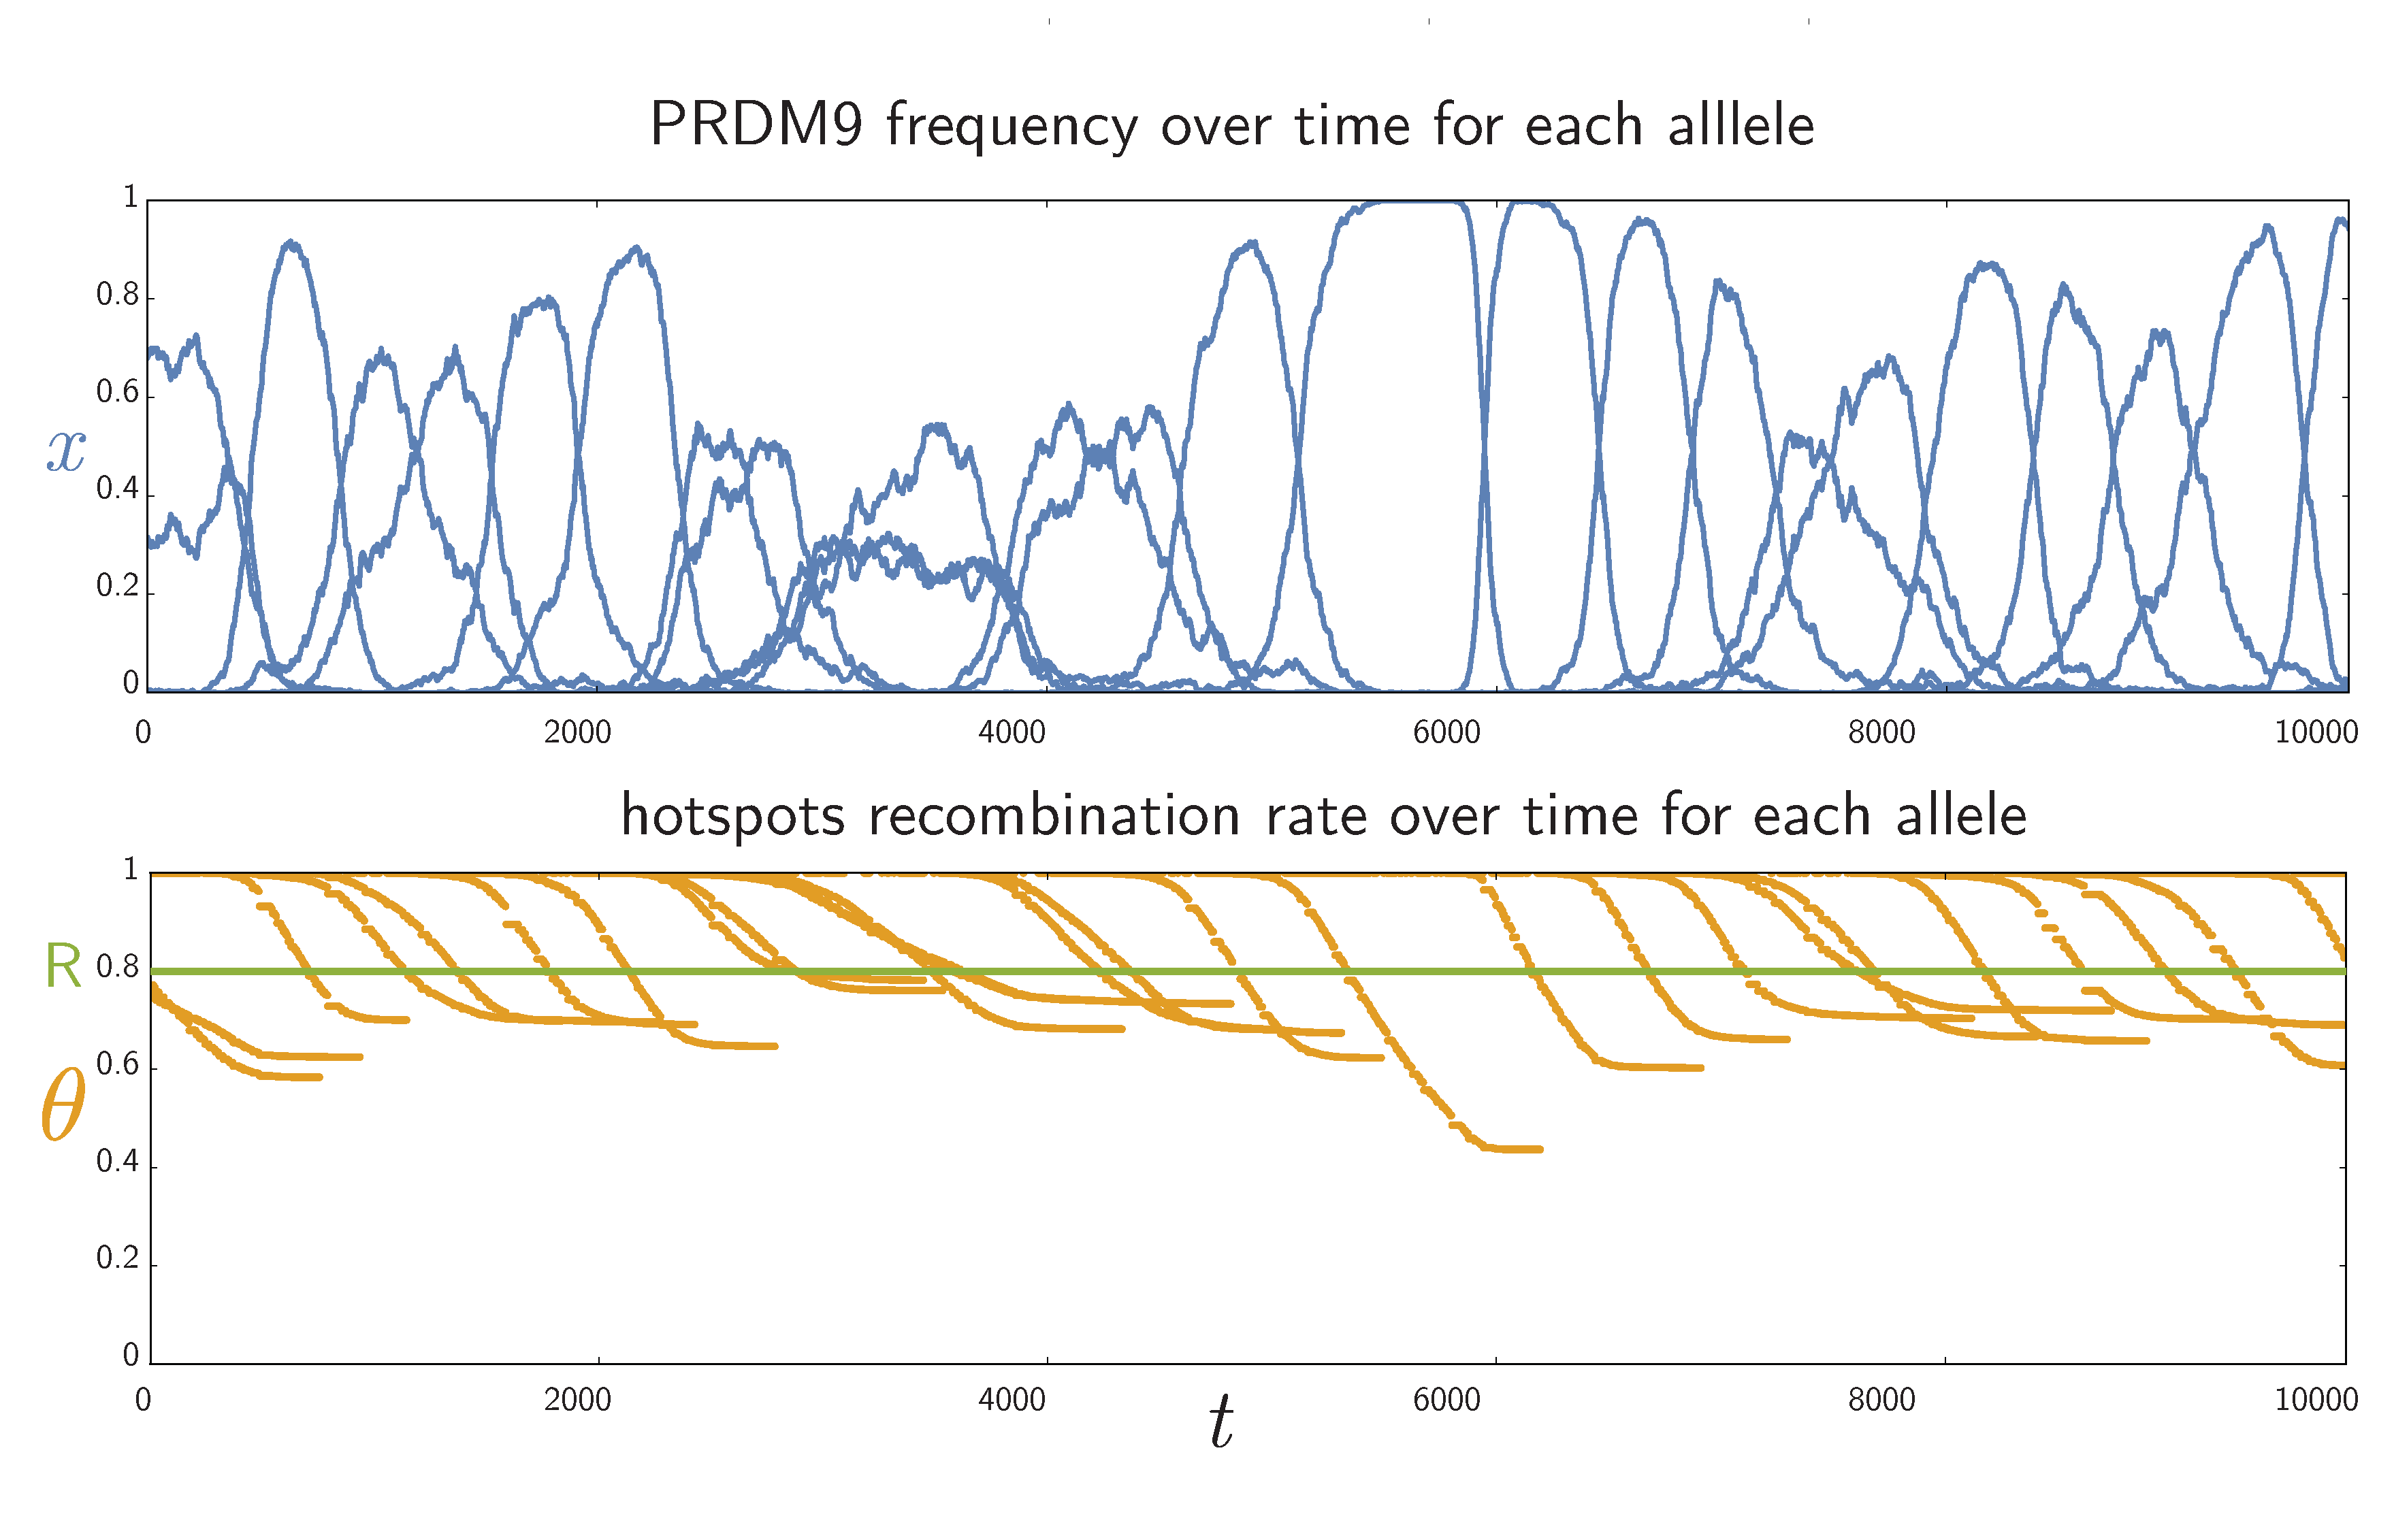
\includegraphics[width=0.8\textwidth]{Images/simulated-trajectory.pdf}\\
\end{figure*}
\textbf{Figure 1.} A typical simulation trajectory of the Red Queen model, with allele frequencies (top) and allele activity (bottom) through time.

\newpage

\begin{figure*}[!ht]
	  \centering
       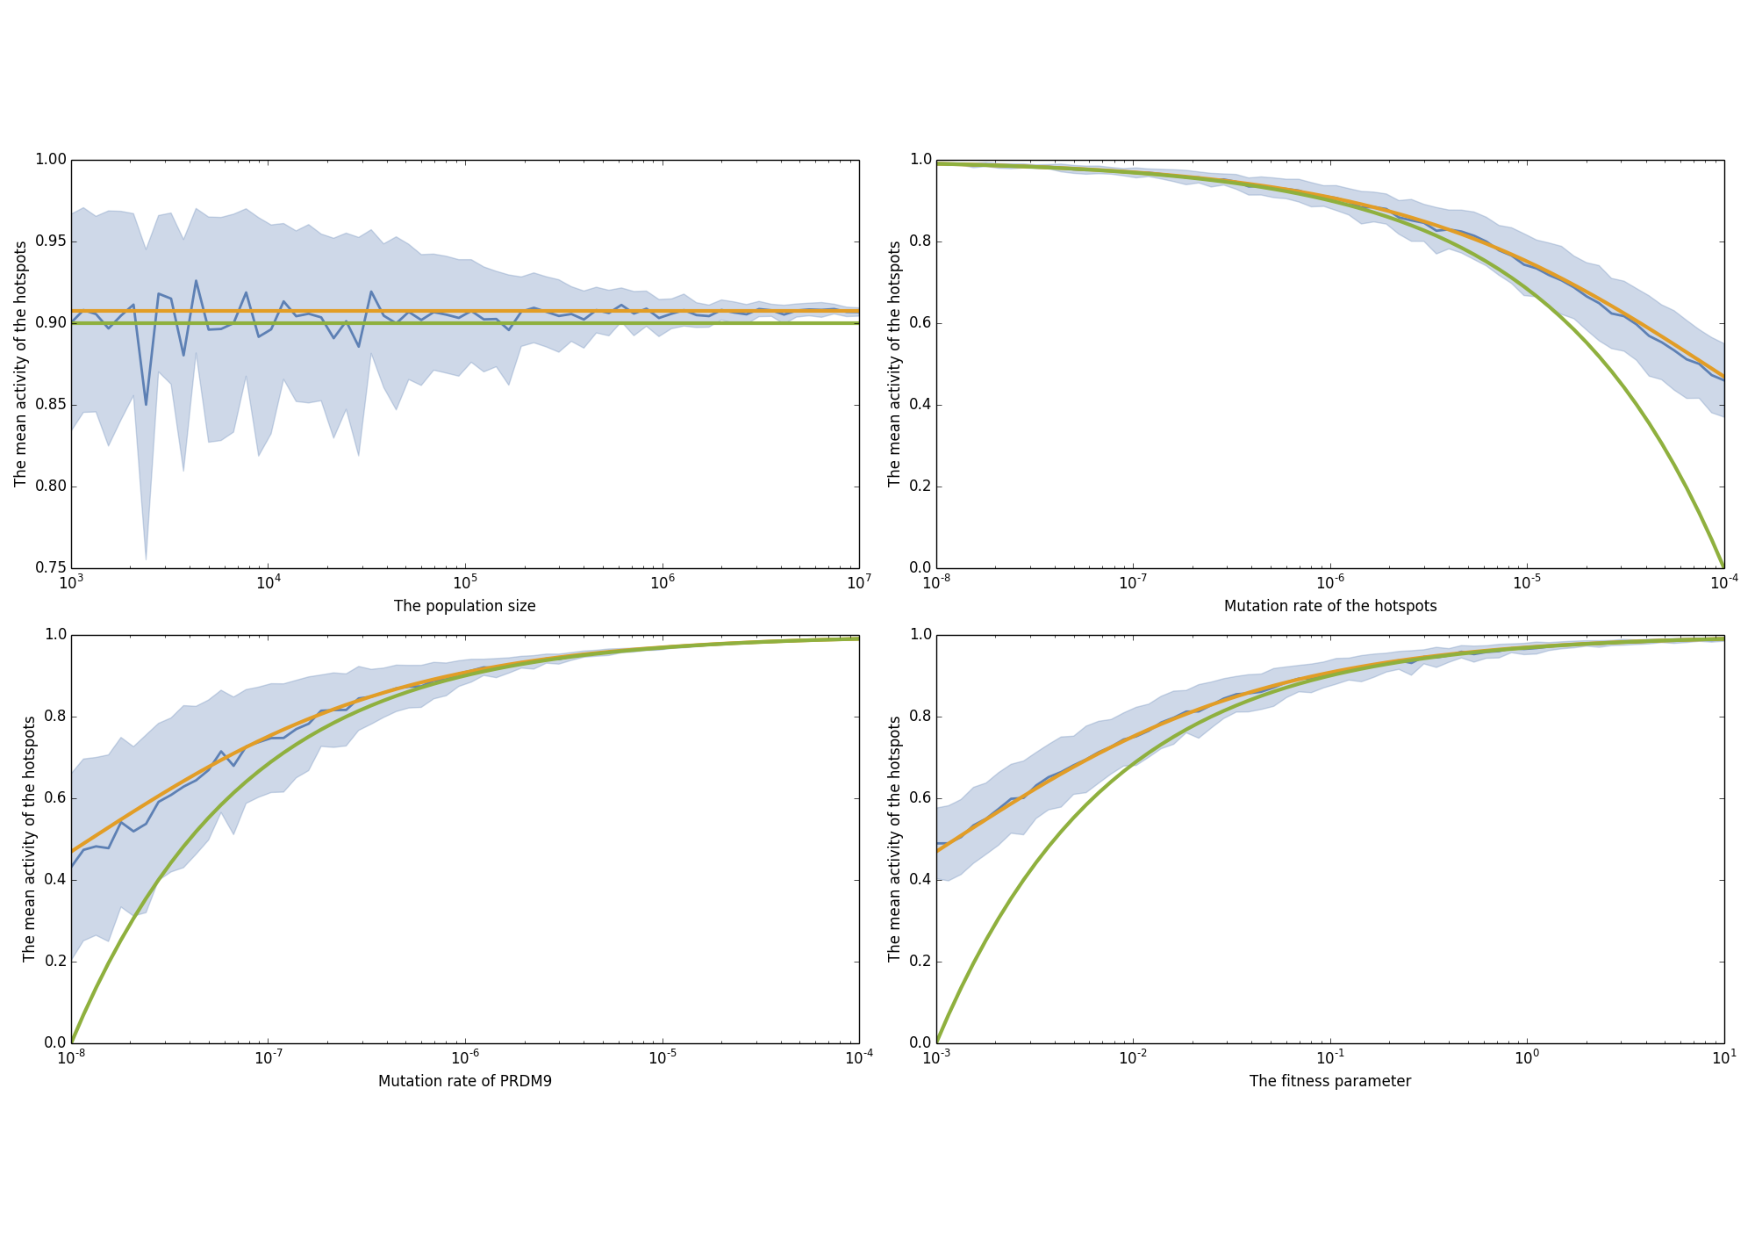
\includegraphics[width=0.8\textwidth]{Images/mean-activity.pdf}\\
\end{figure*}
\textbf{Figure 2.} Mean activity $\R$, as a function of effective population size $N_e$ (top left), mutation rate at the targets $v$ (top right), mutation rate at the PRDM9 locus $u$ (bottom left) and selection strength $\alpha$ (bottom right). Mean-field approximation (orange) and small-load approximation (green).

\newpage

\begin{figure*}[!ht]
	  \centering
       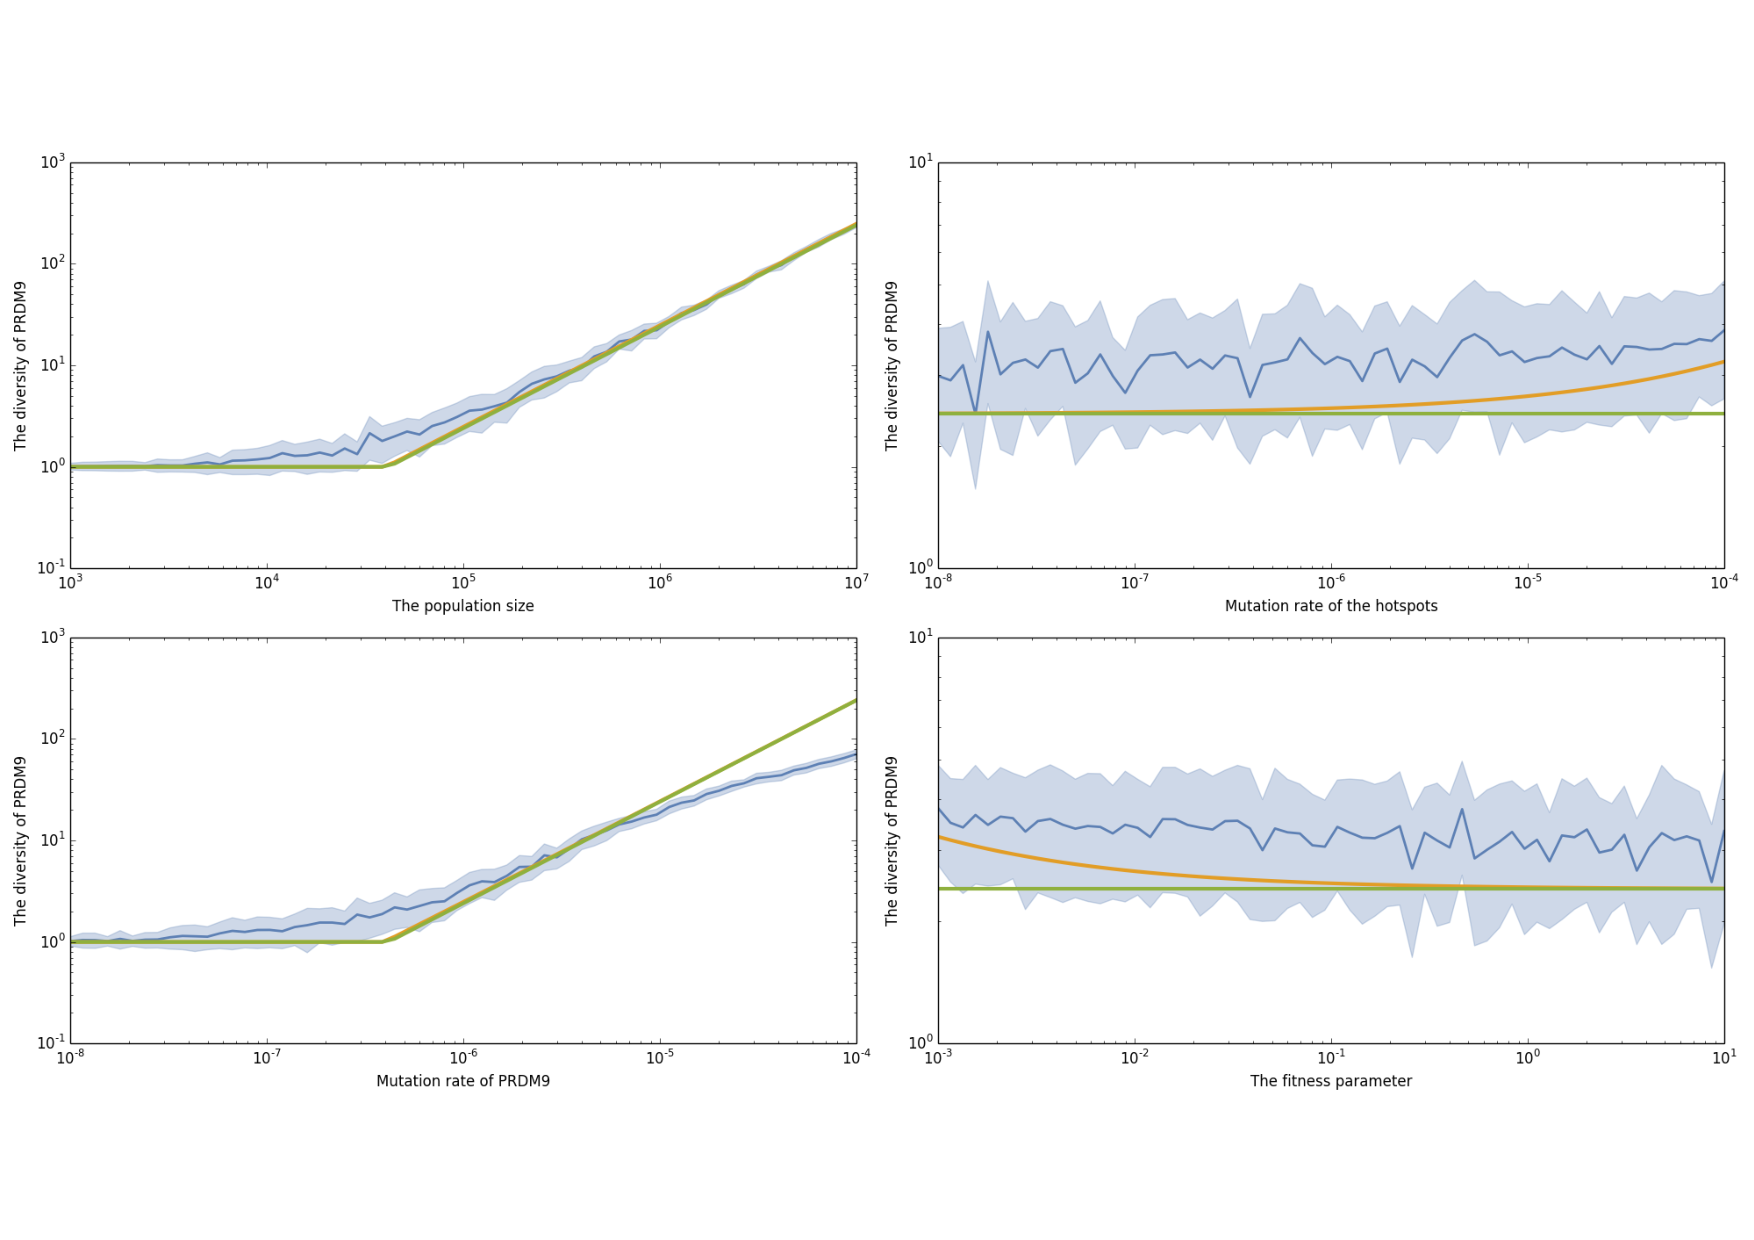
\includegraphics[width=1.0\textwidth]{Images/prdm9-diversity.pdf}\\
\end{figure*}
\textbf{Figure 3.} Diversity at the PRDM0 locus $\D$, as a function of effective population size $N_e$ (top left), mutation rate at the targets $v$ (top right), mutation rate at the PRDM9 locus $u$ (bottom left) and selection strength $\alpha$ (bottom right). Mean-field approximation (orange) and small-load approximation (green).

\newpage

\begin{figure*}[!ht]
	  \centering
       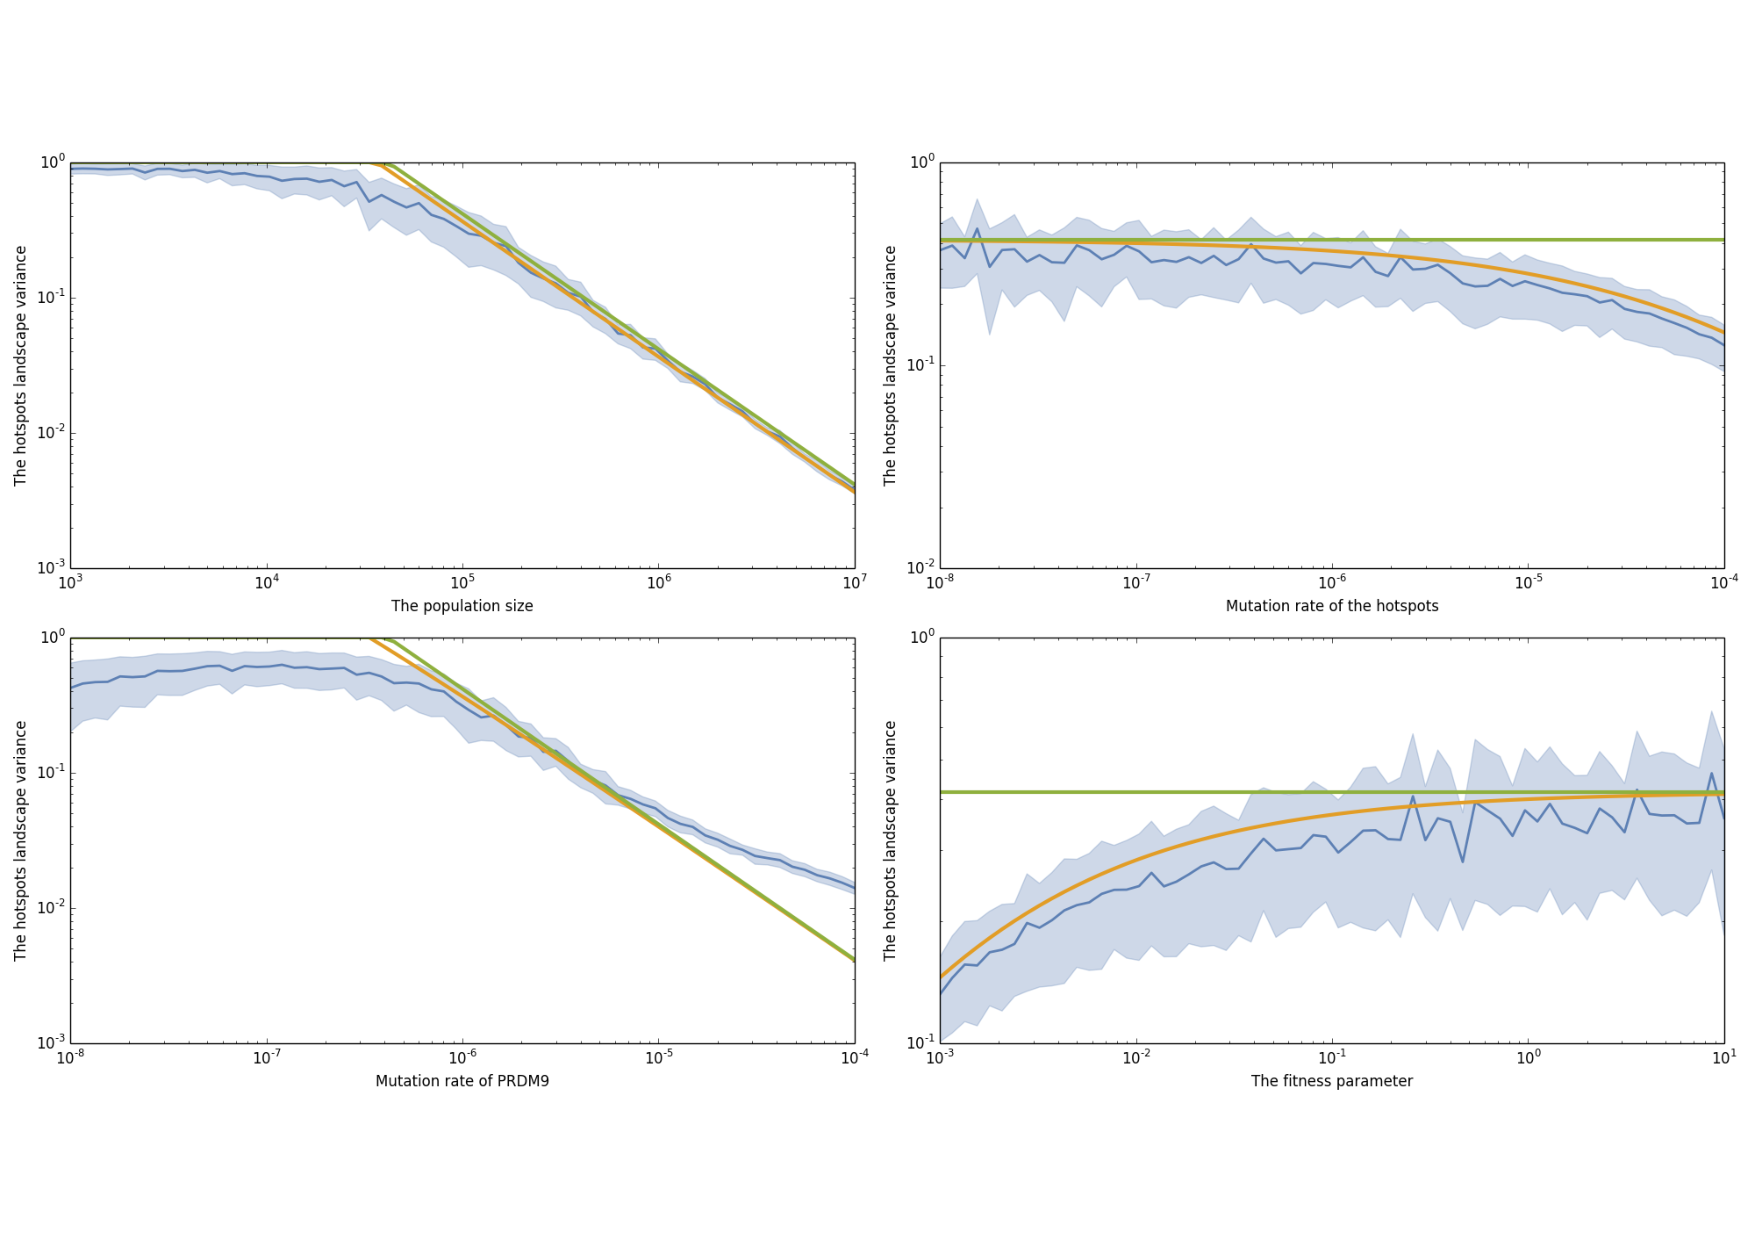
\includegraphics[width=1.0\textwidth]{Images/landscape-variance.pdf}\\
\end{figure*}
\textbf{Figure 4.} Relative variance of recombination landscapes $\V$, as a function of effective population size $N_e$ (top left), mutation rate at the targets $v$ (top right), mutation rate at the PRDM9 locus $u$ (bottom left) and selection strength $\alpha$ (bottom right). Mean-field approximation (orange) and small-load approximation (green).

\newpage

\begin{figure*}[!ht]
	  \centering
       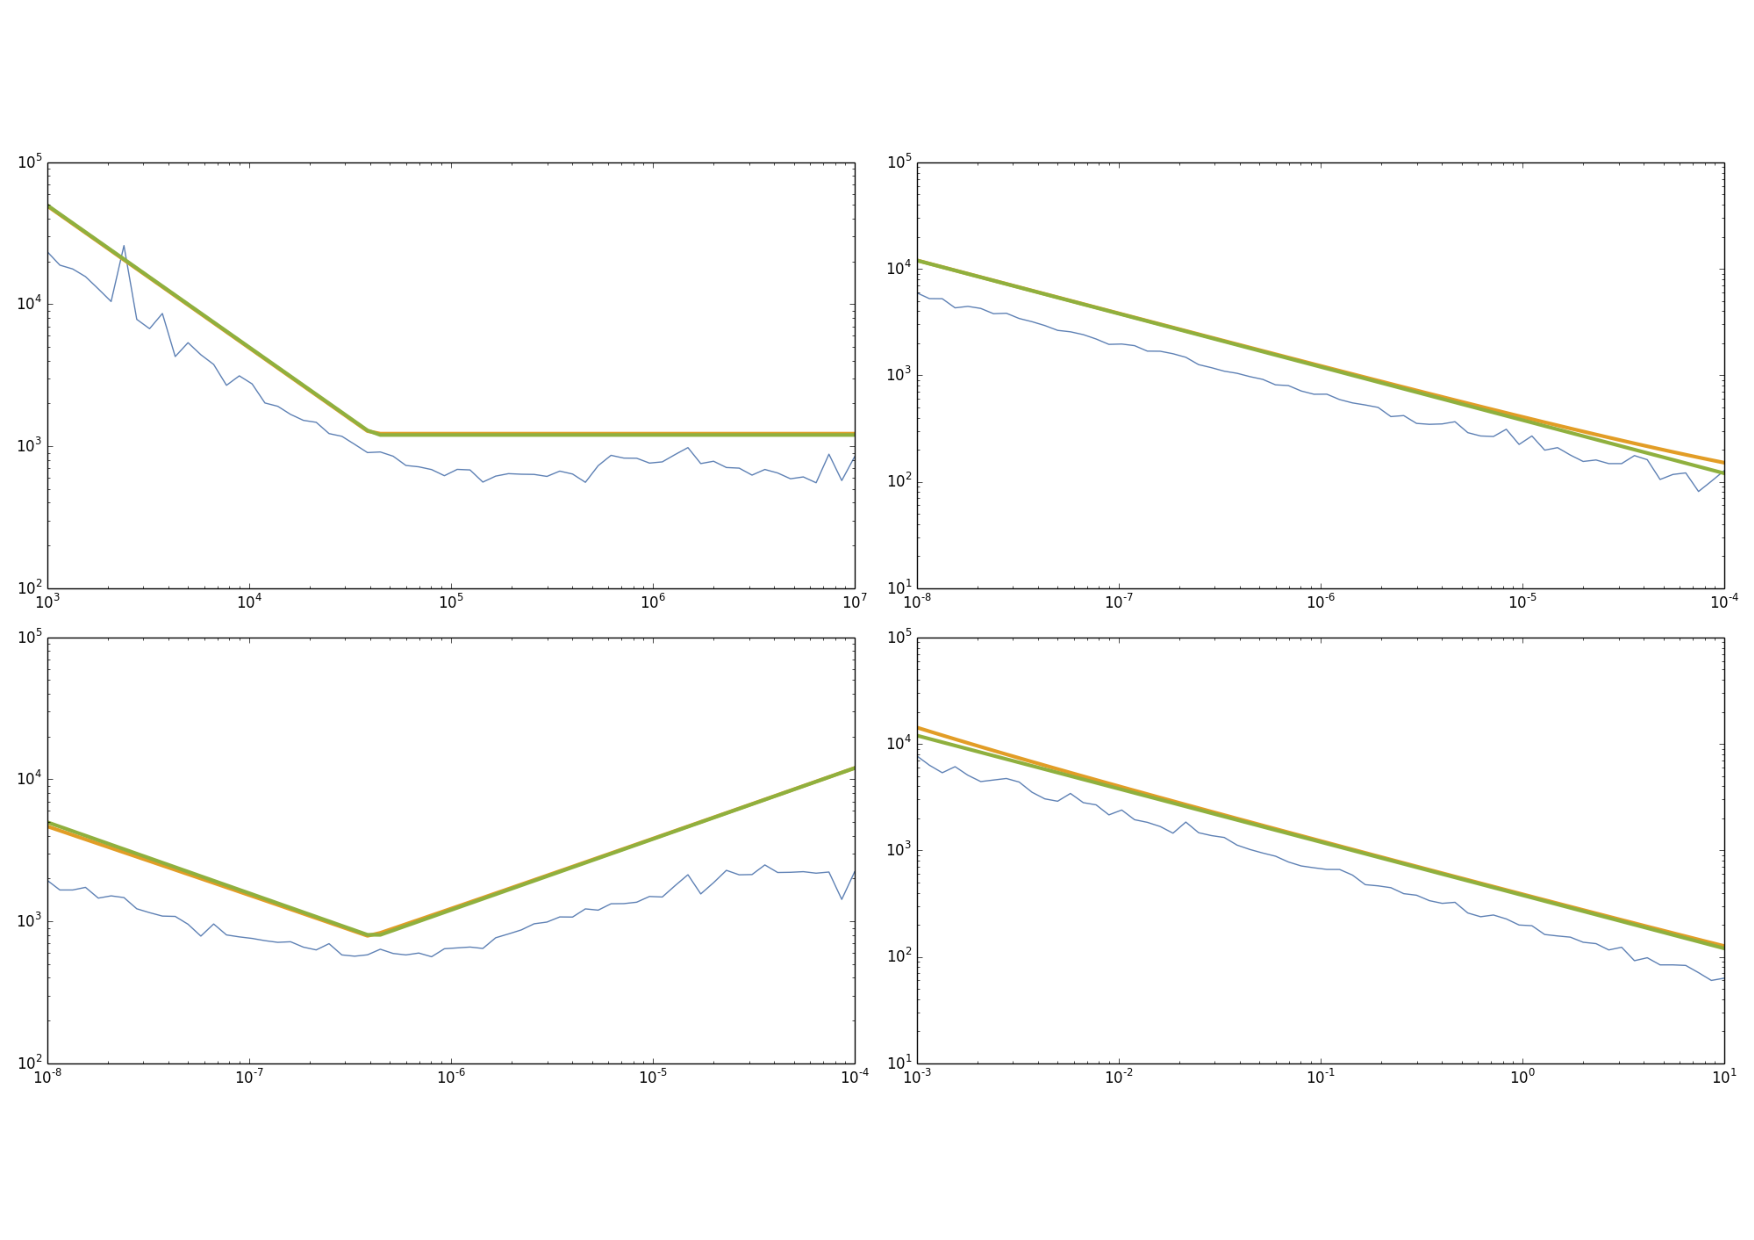
\includegraphics[width=1.0\textwidth]{Images/turn-over.pdf}\\
\end{figure*}
\textbf{Figure 5.} Turnover time $\T$, as a function of effective population size $N_e$ (top left), mutation rate at the targets $v$ (top right), mutation rate at the PRDM9 locus $u$ (bottom left) and selection strength $\alpha$ (bottom right). Mean-field approximation (orange) and small-load approximation (green).

\newpage

\begin{figure*}[!ht]
	  \centering
       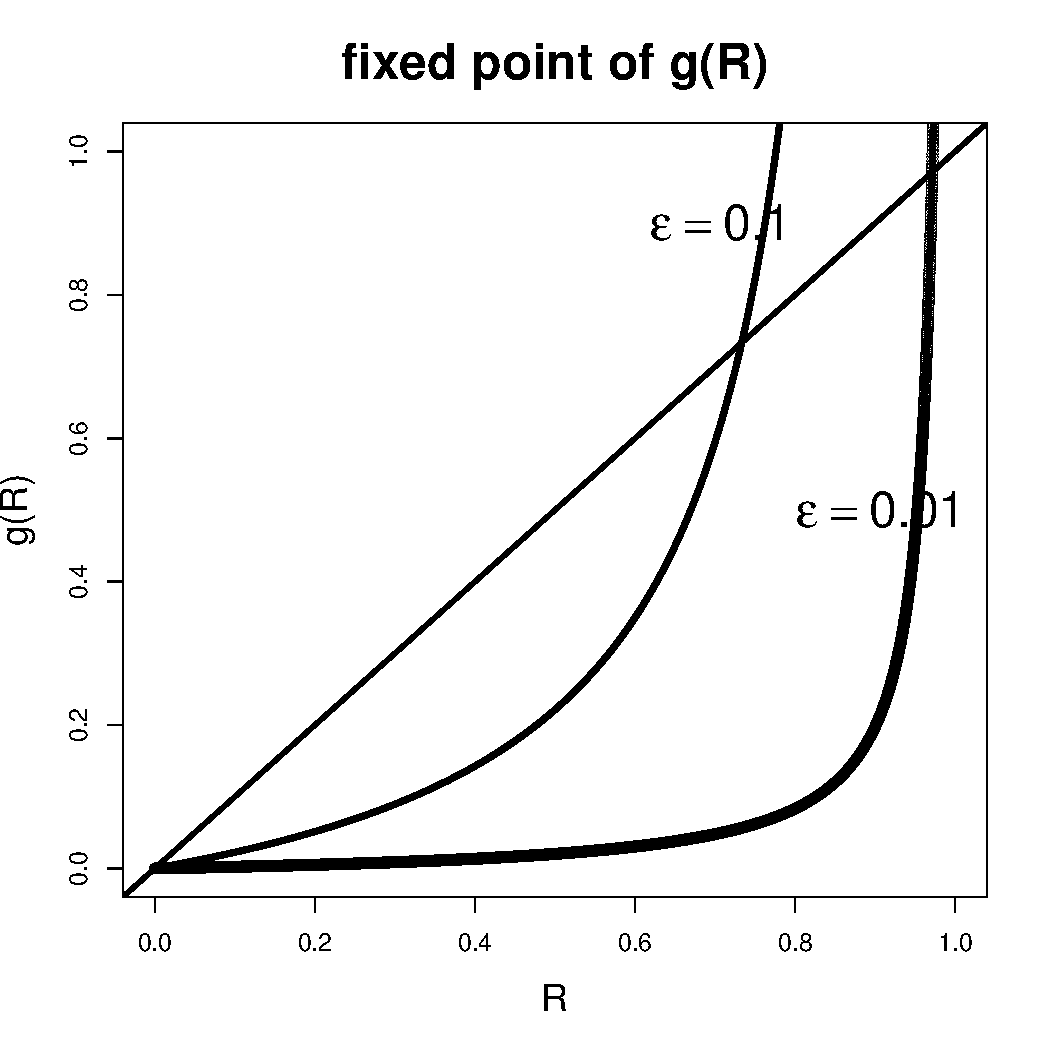
\includegraphics[width=0.8\textwidth]{Images/fixedpoint.pdf}\\
\end{figure*}
\textbf{Figure 6.} Self-consistent solution as a fixed point, in the form $R = g(R)$, for two values of $\epsilon = \sqrt{\dfrac{v r_0}{\alpha u}}$.

%\newpage

%\textbf{Figure 6.} Allele frequency ($x_t$) as a function of activity ($\theta_t$).

\newpage

\begin{figure*}[!ht]
	  \centering
       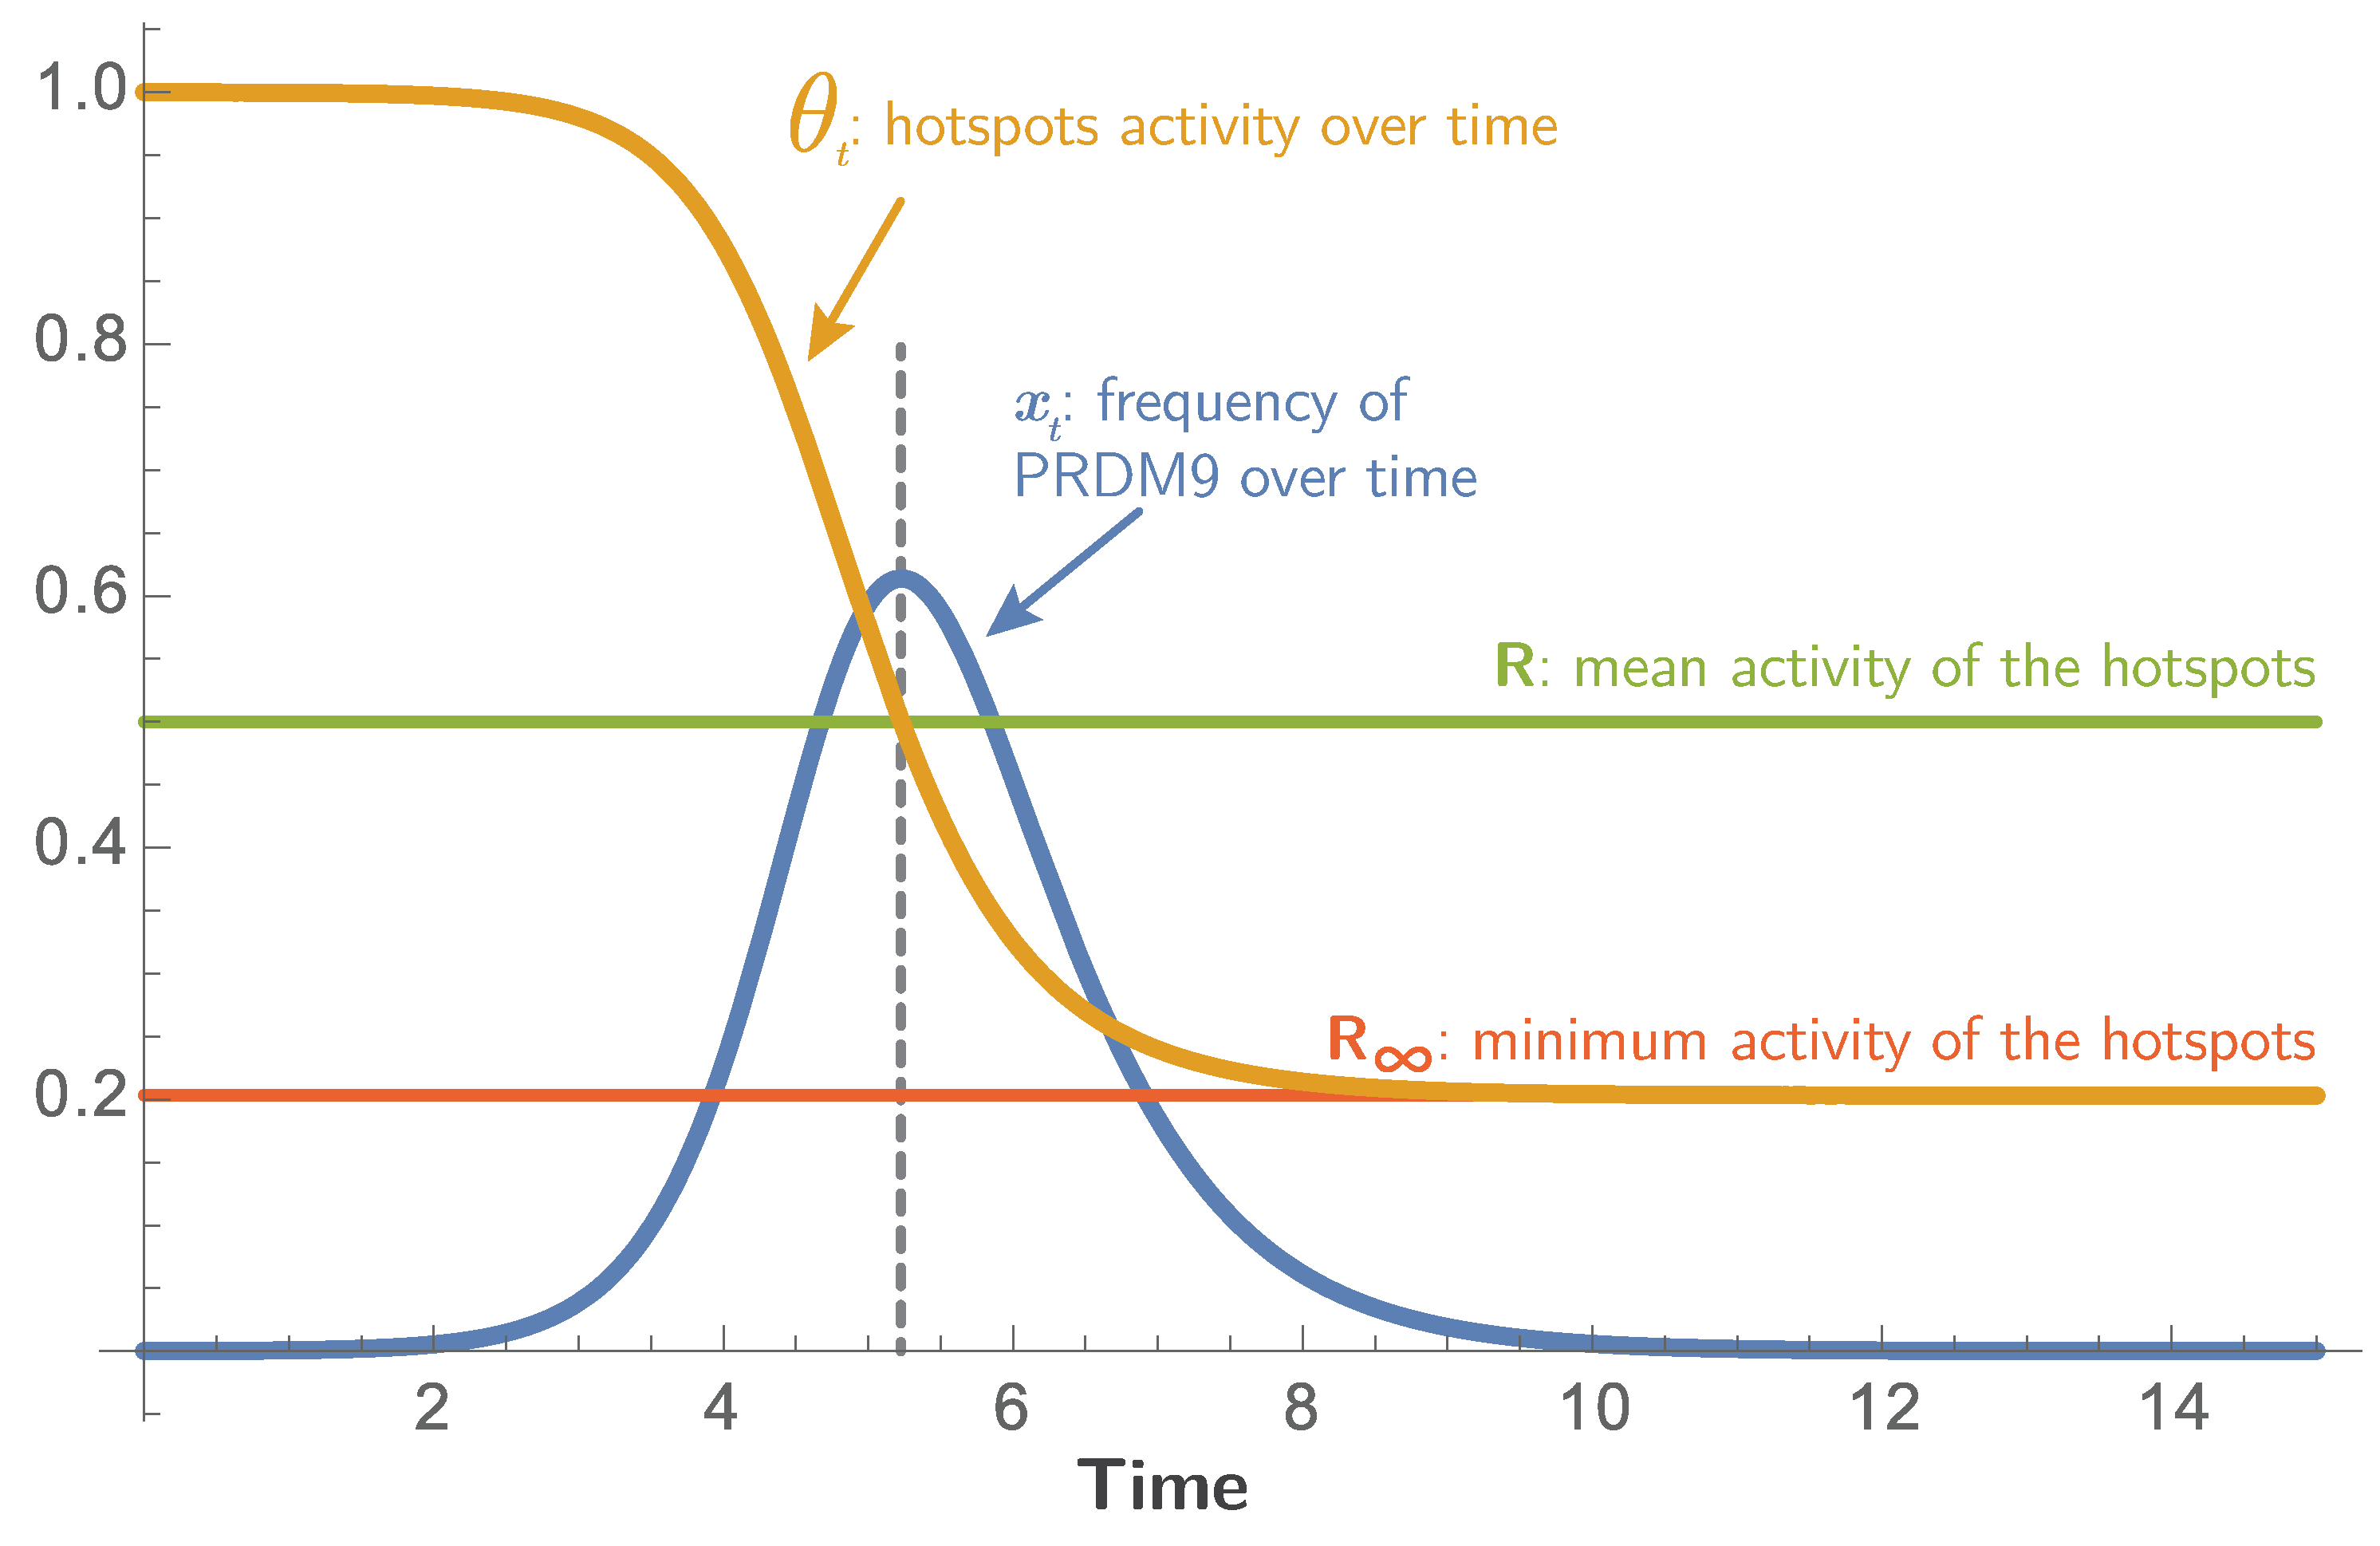
\includegraphics[width=0.8\textwidth]{Images/single-allele.pdf}\\
\end{figure*}
\textbf{Figure 7.} Trajectory of the frequency and the activity of a typical allele through time, under the deterministic and mean-field approximation (see text for details).

%\newpage

%\textbf{Figure 6.} Allele frequency ($x_t$) as a function of activity ($\theta_t$).

\newpage

\begin{figure*}[!ht]
	  \centering
       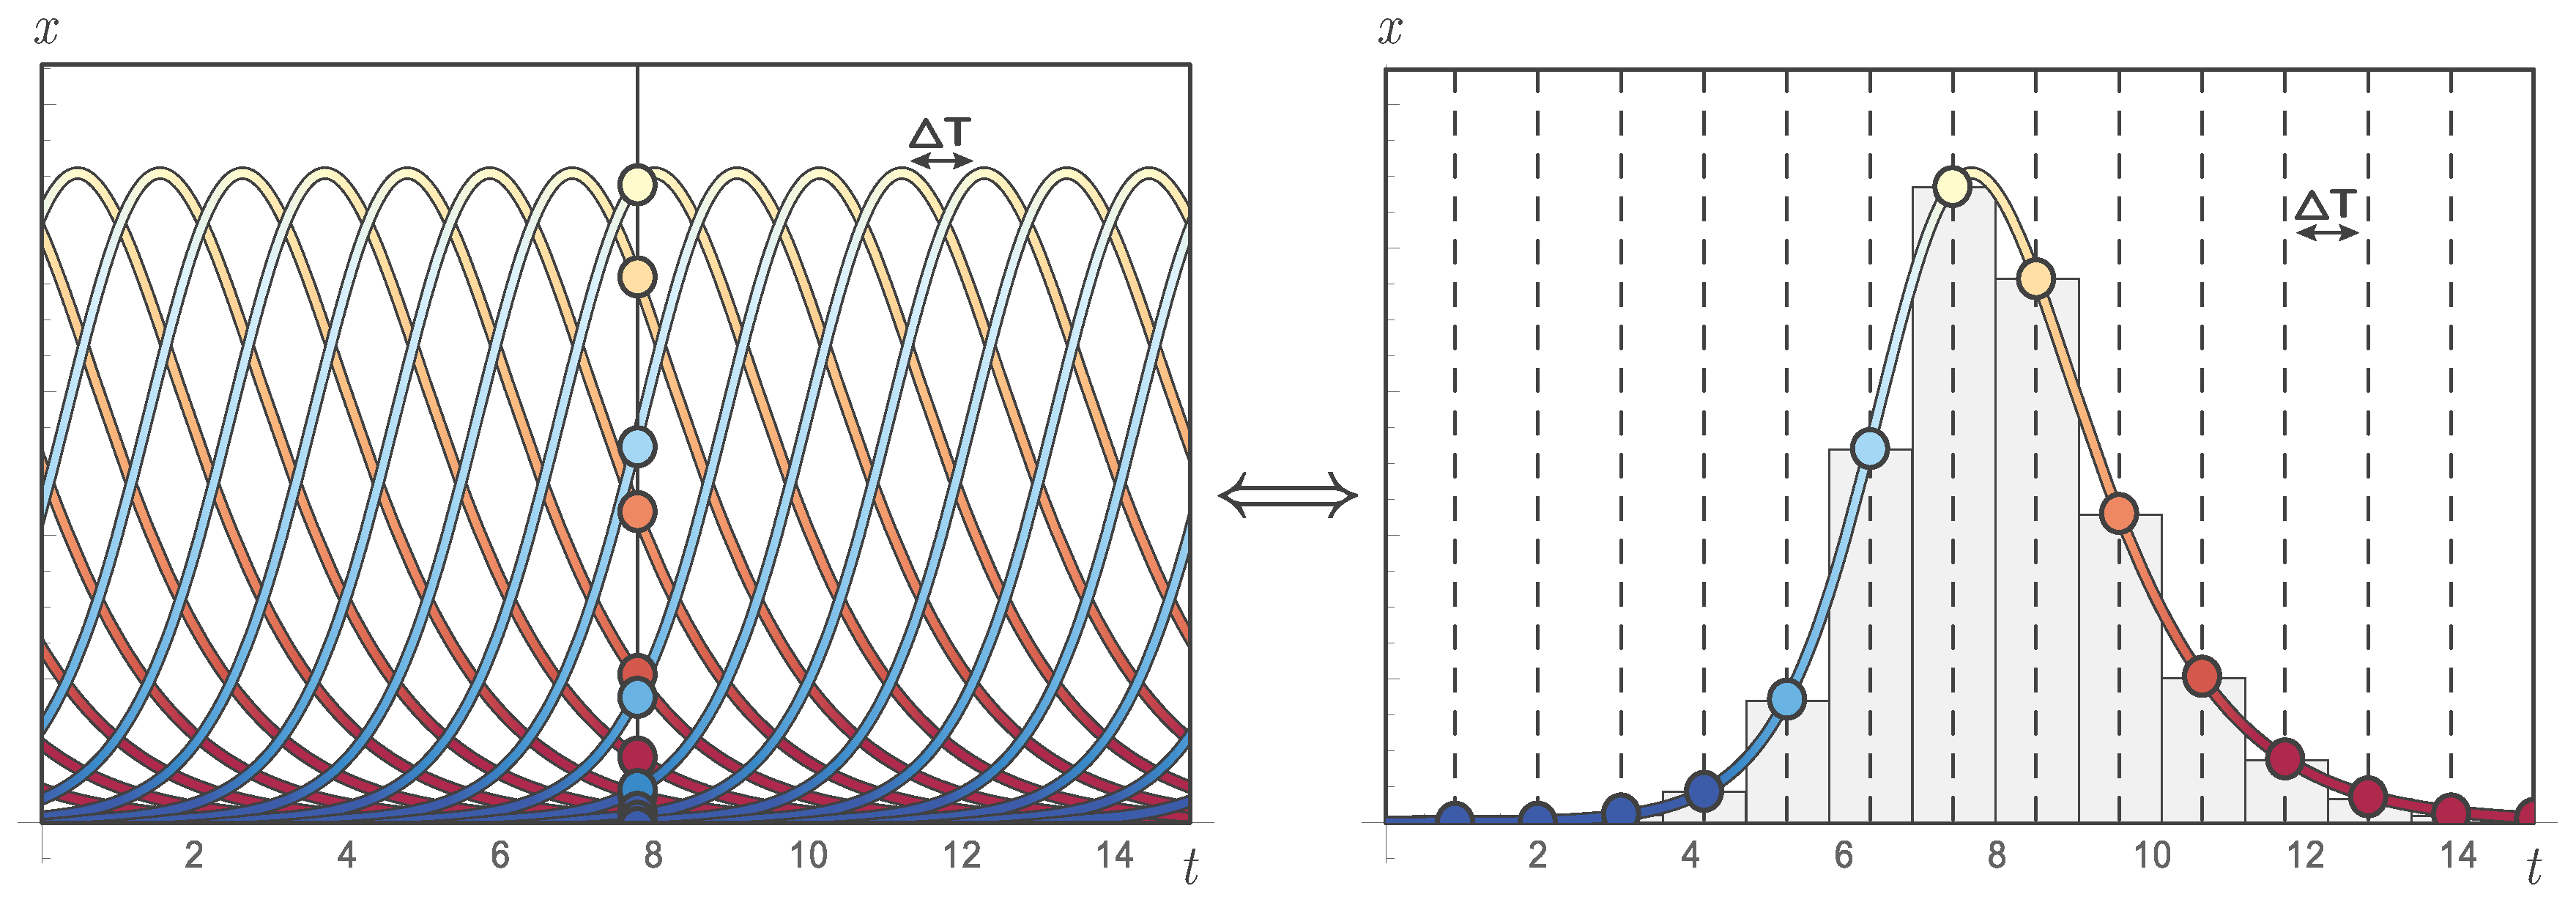
\includegraphics[width=0.8\textwidth]{Images/tilling-argument.pdf}\\
\end{figure*}
\textbf{Figure 8.} A tiling principle. On the left, an idealized realization of the Red Queen dynamic is depicted, in which new alleles invade the population at regular time intervals, all equal to $\tau$, and have the same allele frequency trajectory (such as depicted in figure 6). Taking the sum of allele frequencies at any given time (vertical bar), which by definition is equal to 1, is then equivalent to summing the values taken by the frequency of one specific allele at regular time intervals (right). Multiplying this sum by $\tau$ amounts to approximating the integral $\int x_t d_t$ by the histogram shown on the right panel. Thus, $\int x_t dt \simeq \tau \sum x_i = \tau$. This argument can more generally be used to approximate sums of the form $\sum x_i^k \theta_i^l$ by the corresponding integrals, $\frac{1}{\tau} \left( \int x_t^k \theta_t^l dt \right)$, all of which are analytically available.

\newpage

\part*{Appendix}
\section*{Approximation for the fitness function}
Let us define $\R_{t} =\sum_{i  \in K_{t}} x_{i,t} \Rp _{i,t}$.

One can use a Taylor approximation to linearise the fitness function around $\R $.  

\begin{align}
    \overline{\omega_{i,t}} - f(\R_{t} ) &=
    \sum_{j \in K_{t}} x_{j,t} f \left( \dfrac{\Rp _{i,t} + \Rp _{j,t}}{2} \right) - \sum_{j \in K_{t}} x_{j,t} f(\R_{t} ) \\
    &=
    \sum_{j \in K_{t}} x_{j,t}  \left[ f \left( \dfrac{\Rp _{i,t} + \Rp _{j,t}}{2} \right) - f(\R_{t} ) \right] \\
    &\simeq
    \sum_{j \in K_{t}} x_{j,t}  f'(\R_{t} ) \left( \dfrac{\Rp _{i,t} + \Rp _{j,t}}{2} - \R_{t}  \right) \\
    &\simeq
     f'(\R_{t} ) \left( \dfrac{\Rp _{i,t} + \sum_{j \in K_{t}} x_{j,t} \Rp _{j,t}}{2} - \R_{t}  \right) \\
     &\simeq
     f'(\R_{t} ) \left( \dfrac{\Rp _{i,t} - \R_{t} }{2}\right) \\
\end{align}

Consequently $\overline{\omega_{t}} \simeq f(\R_{t} )$. \textbf{Proof},

\begin{align}
    f(\R_{t} ) &= \sum_{i \in K_{t}} x_{i,t} f(\R_{t} ) \\
    &\simeq \sum_{i \in K_{t}} x_{i,t} \left[ \overline{\omega_{i,t}} - f'(\R_{t} ) \left( \dfrac{\Rp _{i,t} - \R_{t} }{2}\right) \right] \\
    &\simeq
    \sum_{i \in K_{t}} x_{i,t} \overline{\omega_{i,t}} - f'(\R_{t} ) \sum_{i \in K_{t}} x_{i,t}  \left( \dfrac{\Rp _{i,t} - \R_{t} }{2}\right) \\
    &\simeq
     \overline{\omega_{t}} - f'(\R_{t} )  \left( \dfrac{\sum_{i \in K_{t}} x_{i,t} \Rp _{i,t} - \R_{t} }{2}\right) \\
    &\simeq
     \overline{\omega_{t}}
\end{align}

And the selection coefficient $s_{i,t}$ for the allele $i$ can be easily computed

\begin{equation}
    s_{i,t} = \dfrac{\overline{\omega_{i,t}} - \overline{\omega_{t}}}{\overline{\omega_{t}}}
    \simeq  \dfrac{f'(\R_{t} )}{f(\R_{t} )} \left[ \dfrac{\Rp _{i,t} - \R_{t} }{2} \right]
\end{equation}

\section*{Analytical relation between frequency and activity in the polymorphic regime.}

\begin{align} 
& \left\{
      \begin{aligned}
          \dfrac{\dd x_{t}}{\dd t} &= \dfrac{f'(\R )}{2 f(\R )} \left( \Rp_{t}  - \R \right) x_{t} \\
        \dfrac{\dd \Rp_{t}}{\dd t} &= 
        - \rho x_{t} \Rp_{t} \\
      \end{aligned}
\right. \\
 \Rightarrow
 & \left\{
      \begin{aligned}
          \dfrac{\dd x_{t}}{\dd \Rp_{t} } &= \dfrac{f'(\R )}{2 \rho f(\R )}\left( \dfrac{\R }{\Rp_{t} } -1 \right) \\
        \dfrac{\dd \Rp_{t} }{\dd t} &= 
        - \rho x_{t} \Rp_{t} \\
      \end{aligned}
    \right. \\
 \Rightarrow
  & \left\{
      \begin{aligned}
         x(\Rp_{t} ) &=\dfrac{f'(\R)}{2 \rho f(\R )} (1- \Rp_{t}  + \R  \operatorname{log}(\Rp_{t} )) + x_{\mathrm{initial}}  \\
        \dfrac{\dd \Rp_{t} }{\dd t} &= 
         \dfrac{f'(\R )}{2 f(\R )} [ \Rp_{t} -1- \R  \operatorname{log}(\Rp_{t} )]\Rp_{t}   - \rho x_{\mathrm{initial}} \Rp_{t} \\
      \end{aligned}
    \right.
\end{align}

\section*{$\tau$, $\D$ and $\V$ in polymorphic regime.}
We make use of the three equations :  
\begin{equation}
\left\{
  \begin{aligned}
         x(\Rp_{t} ) &= \dfrac{f'(\R)}{2 \rho f(\R )} (1- \Rp_{t}  + \R  \operatorname{log}(\Rp_{t} )) \\
         \dfrac{\dd t }{\dd \Rp_{t}} &= \dfrac{1}{-\rho x_{t} \Rp_{t}} \\
        0 &= 1-\Rmin  + \R  \operatorname{log}(\Rmin )  \\
  \end{aligned}
   \right.
\end{equation}

\begin{align}
\tau &= \int_{0}^{\infty } x_{t} \dd t  \\
    &= \int_{1}^{\Rmin } x(\Rp_{t} )   \dfrac{\dd t }{\dd  \Rp_{t}} \dd \Rp_{t}    \\
    &= \int_{1}^{\Rmin } x(\Rp_{t} )   \dfrac{1 }{- \rho x(\Rp_{t} ) \Rp_{t} } \dd \Rp_{t}    \\
    &=  \dfrac{-1 }{\rho }  \int_{1}^{\Rmin }   \dfrac{1 }{\Rp_{t} } \dd \Rp_{t}    \\
    &=  \dfrac{-1 }{\rho } \left[ \operatorname{log}(\Rp_{t}) \right]_{1}^{\Rmin }    \\
    &=  \dfrac{-1 }{\rho } \operatorname{log}(\Rmin )    \\
    &=  \dfrac{1 - \Rmin }{\rho \R } \displaybreak[3] \\ 
\D &= \left( \dfrac{\int_{0}^{\infty } x_{t}^2 \dd  t}{ \tau } \right)^{-1} \\
    &=   \tau \left( \int_{0}^{\infty } x_{t}^2 \dd  t \right)^{-1} \\
    &=   \tau  \left(\int_{1}^{\Rmin } x(\Rp_{t} )^2 \dfrac{\dd t }{\dd  \Rp_{t}} \dd \Rp_{t} \right)^{-1} \\
    &=   \dfrac{ \operatorname{log}(\Rmin ) }{-\rho  }  \left( \int_{1}^{\Rmin } x(\Rp_{t} )^2 \dfrac{1 }{- \rho x(\Rp_{t} ) \Rp_{t} } \dd \Rp_{t} \right)^{-1} \\
    &=   \operatorname{log}(\Rmin ) \left( \int_{1}^{\Rmin } \dfrac{x(\Rp_{t} ) }{ \Rp_{t} } \dd \Rp_{t} \right)^{-1} \\ 
    &=  \operatorname{log}(\Rmin ) \left( \int_{1}^{\Rmin } \dfrac{f'(\R)}{2 \rho f(\R )} \dfrac{ 1- \Rp_{t}  + \R  \operatorname{log}(\Rp_{t} ) }{ \Rp_{t} } \dd \Rp_{t} \right)^{-1} \\ 
    &=  \dfrac{2 \rho f(\R )}{f'(\R)} \operatorname{log}(\Rmin ) \left( \left[  - \Rp_{t} + \operatorname{log}(\Rp_{t}) + \dfrac{\R \operatorname{log}(\Rp_{t})^2}{2}  \right]_{1}^{\Rmin } \right)^{-1} \\ 
	&=  \dfrac{2 \rho f(\R )}{f'(\R)} \operatorname{log}(\Rmin ) \left( 1 - \Rmin + \operatorname{log}(\Rmin) + \dfrac{\R \operatorname{log}(\Rmin)^2}{2} \right)^{-1} \\ 
	&=  \dfrac{2 \rho f(\R )}{f'(\R)} \operatorname{log}(\Rmin ) \left( -\R \operatorname{log}(\Rmin) + \operatorname{log}(\Rmin) + \dfrac{\R \operatorname{log}(\Rmin)^2}{2} \right)^{-1} \\ 
	&=  \dfrac{2 \rho f(\R )}{f'(\R)}  \left(   -\R + 1 + \dfrac{\R \operatorname{log}(\Rmin)}{2}  \right)^{-1} \\ 
	&=  \dfrac{2 \rho f(\R )}{f'(\R)}  \left(  \dfrac{ -2\R + 2 + \Rmin - 1 }{2}  \right)^{-1} \\ 
    &= \dfrac{4 \rho f(\R )}{f'(\R )\left[ 1 + \Rmin  - 2 \R   \right]} \displaybreak[3] \\ 
\V &= \dfrac{\int_{0}^{\infty } x_{t}^2  \Rp_{t} \dd  t}{ \tau }  \\
    &=   \dfrac{1}{\tau} \int_{1}^{\Rmin } x(\Rp_{t} )^2 \Rp_{t} \dfrac{\dd t }{\dd  \Rp_{t}} \dd \Rp_{t}  \\
    &=  \dfrac{ \rho \R }{1 - \Rmin }  \int_{1}^{\Rmin } x(\Rp_{t} )^2 \Rp_{t} \dfrac{1 }{- \rho x(\Rp_{t} ) \Rp_{t} } \dd \Rp_{t}  \\
    &=   \dfrac{ \R }{\Rmin - 1} \int_{1}^{\Rmin } x(\Rp_{t} )  \dd \Rp_{t} \\ 
    &=   \dfrac{ \R }{\Rmin - 1} \int_{1}^{\Rmin } \dfrac{f'(\R)}{2 \rho f(\R )} [ 1- \Rp_{t}  + \R  \operatorname{log}(\Rp_{t} )  ] \dd \Rp_{t} \\ 
    &=  \dfrac{f'(\R)}{2 \rho f(\R )} \dfrac{ \R }{\Rmin - 1} \left[  \Rp_{t} - \dfrac{\Rp_{t}^2}{2} - \Rp_{t} \R + \Rp_{t} \R \operatorname{log}(\Rp_{t} )   \right]_{1}^{\Rmin }  \\ 
	&=  \dfrac{f'(\R)}{2 \rho f(\R )} \dfrac{ \R }{\Rmin - 1} \left(  R - \dfrac{1}{2} + \Rmin - \dfrac{\Rmin^2}{2} - \Rmin \R + \Rmin \R \operatorname{log}(\Rmin )   \right)  \\
	&=  \dfrac{f'(\R)}{2 \rho f(\R )} \dfrac{ \R }{\Rmin - 1} \dfrac{ 2 R - 1 + 2\Rmin - \Rmin^2 - 2 \Rmin \R + 2 \Rmin (\Rmin - 1 )  }{2}  \\
	&=  \dfrac{f'(\R)}{2 \rho f(\R )} \dfrac{ \R }{\Rmin - 1} \left( 2 R - \Rmin - 1  + \Rmin + \Rmin^2 - 2 \Rmin \R \right)  \\
	&=  \dfrac{f'(\R)}{2 \rho f(\R )} \dfrac{ \R }{\Rmin - 1} (\Rmin - 1 )\left(  1 + \Rmin  - 2 \R \right)  \\
	&= \dfrac{f'(\R )}{4 \rho f(\R )}\R \left[ 1 + \Rmin  - 2 \R   \right] 
\end{align}

\section*{Small load development}


The first approximation is to set a power law function for the fitness; $f(x)=x^{\alpha}$, thus $f'(\R)/f(\R)= \alpha / \R$.


Let us define $\epsilon =  \sqrt{\dfrac{ \rho }{ \alpha \mu }} = \sqrt{\dfrac{v r_0}{\alpha u}}$

Let us define $\Lr = 1 - \R $ is the recombination gap and $\Lmin = 1 - \Rmin $ is the maximum recombination gap.
We make as second order development on $\epsilon$ for both $\Lr$ and $\Lmin$
\begin{align}
&\left\{
  \begin{aligned}
         \Lr &= \Lra \epsilon + \Lrb \epsilon^2 + \circ ( \epsilon^2) \\
         \Lmin &= \Lmina \epsilon + \Lminb \epsilon^2 + \circ ( \epsilon^2)  \\
  \end{aligned}
   \right.
   \\ \Rightarrow
&\left\{
  \begin{aligned}
         \Lr^2 &= \Lra^2 \epsilon^2 + \circ ( \epsilon^2) \\
         \Lmin^2 &= \Lmina^2 \epsilon^2 + \circ ( \epsilon^2)  \\
         \Lmin \Lr&= \Lmina \Lra \epsilon^2 + (\Lmina \Lrb + \Lminb \Lra)  \epsilon^3 + \circ ( \epsilon^3)   \\
  \end{aligned}
   \right.
\end{align}

\begin{align}
&\left\{
  \begin{aligned}
         0 &= 1-\Rmin  + \R  \operatorname{log}(\Rmin ) \\
         \epsilon^2 &=  \dfrac{(1- \R )(1- \Rmin )}{2 \R^2} 
  \end{aligned}
   \right.
   \\ \Rightarrow
&\left\{
  \begin{aligned}
         0 &= \Lmin  + ( 1- \Lr) \operatorname{log}(1 - \Lmin ) \\
         \epsilon^2 &=  \dfrac{ \Lmin \Lr }{2(1- \Lr)^2} 
  \end{aligned}
   \right.
    \\ \Rightarrow
   &\left\{
  \begin{aligned}
       &  -\Lmin = ( 1- \Lr) \left(-\Lmin - \dfrac{\Lmin^2}{2} - \dfrac{\Lmin^3}{3} + \circ ( \Lmin^3) \right) \\
       &   \Lmin \Lr =   2 (1- \Lr)^2 \epsilon^2
  \end{aligned}
   \right.
       \\ \Rightarrow
   &\left\{
  \begin{aligned}
       &  1 = ( 1- \Lr) \left(1 + \dfrac{\Lmin}{2} + \dfrac{\Lmin^2}{3} + \circ ( \Lmin^2) \right) \\
       &   \Lmin \Lr =  2 (1- \Lr)^2 \epsilon^2
  \end{aligned}
   \right.
  \\ \Rightarrow
   &\left\{
  \begin{aligned}
       &  1 = [ 1- \Lra \epsilon - \Lrb \epsilon^2 + \circ ( \epsilon^2) ] \left(1 + \dfrac{\Lmina \epsilon }{2} + \dfrac{ \Lminb \epsilon^2}{2}  + \dfrac{\Lmina^2 \epsilon^2}{3} + \circ ( \epsilon^2) \right) \\
       &   \Lmina \Lra \epsilon^2 + (\Lmina \Lrb + \Lminb \Lra)  \epsilon^3 + \circ ( \epsilon^3) =  2 (1- \Lra \epsilon - \Lrb \epsilon^2 + \circ ( \epsilon^2))^2 \epsilon^2
  \end{aligned}
   \right.
     \\ \Rightarrow
   &\left\{
  \begin{aligned}
       &  1 = 1 + \dfrac{\Lmina - 2 \Lra }{2} \epsilon + \dfrac{ 2 \Lmina^2 - 3 \Lmina \Lra + 3 \Lminb - 6 \Lrb  }{6} \epsilon^2 + \circ ( \epsilon^2)  \\
       &   \Lmina \Lra + (\Lmina \Lrb + \Lminb \Lra)  \epsilon + \circ ( \epsilon) =   2 - 4 \Lra \epsilon + \circ ( \epsilon )
  \end{aligned}
   \right. \displaybreak[3] \\ 
  \\ \Rightarrow
   &\left\{
     \begin{aligned}
       &  0 = \Lmina - 2 \Lra \\
       &  0 = 2 \Lmina^2 - 3 \Lmina \Lra + 3 \Lminb - 6 \Lrb \\
       &  0 = 2 - \Lmina \Lra   \\
       &  0 = \Lmina \Lrb + \Lminb \Lra + 4 \Lra \\
  \end{aligned}
   \right.
     \\ \Rightarrow
   &\left\{
   \begin{aligned}
       &  \Lmina = 2 \\
       &  \Lra = 1 \\
       &  \Lminb = \dfrac{-7}{3}  \\
       &  \Lrb = \dfrac{-5}{6} \\
  \end{aligned}
     \right.
       \\ \Rightarrow
   &\left\{
     \begin{aligned}
     \R  &=  1 - \epsilon + \dfrac{5}{6} \epsilon^2 + \circ ( \epsilon^2)\\
     \Rmin & =  1 - 2 \epsilon + \dfrac{7}{3} \epsilon^2 + \circ ( \epsilon^2)\\
  \end{aligned}
   \right.
\end{align}

1. Estimation of $1 + \Rmin  - 2 \R$ in polymorphic regime

\begin{align}
1 + \Rmin  - 2 \R &= 1 +  1 - 2 \epsilon + \dfrac{7}{3} \epsilon^2 - 2 \left( 1 - \epsilon + \dfrac{5}{6} \epsilon^2 \right) \\
&=  \dfrac{7}{3} \epsilon^2 - \dfrac{5}{3} \epsilon^2 \\
& =  \dfrac{2}{3} \epsilon^2
\end{align}

2. Estimation of $D$ in polymorphic regime

\begin{align}
  \D &= \dfrac{4 \rho f(\R )}{f'(\R )\left[ 1 + \Rmin  - 2 \R   \right]} \\
  &= \dfrac{4\rho  \R}{ \alpha\left[ 1 + \Rmin  - 2 \R   \right]} \\
   & =  \dfrac{6 \rho}{\alpha \epsilon^2} = 24 N_e u
\end{align}

3. Estimation of $V$ in polymorphic regime

\begin{align}
 \V &=  \dfrac{f'(\R )}{4 \rho f(\R )}\R \left[ 1 + \Rmin  - 2 \R   \right] \\
   &= \dfrac{\alpha }{4 \rho }\left[ 1 + \Rmin  - 2 \R   \right] \\
   &= \dfrac{\alpha \epsilon^2 }{6 \rho} = \dfrac{1}{24 N_e u}
\end{align}

4. Estimation of $ T $ in polymorphic regime

\begin{align}
   \T &= \D \left( \mu \alpha \dfrac{1-\R }{ 2 \R }   \right)^{-1} \\
    &=   \dfrac{6 \rho}{\alpha \epsilon^2 } \dfrac{2}{ \mu \alpha \epsilon } \\
    &=   \dfrac{12}{ \alpha  \epsilon } =  12 \sqrt{\dfrac{u }{\alpha v r_0}}
\end{align}


\end{document}


\section*{Discussion}

\subsection*{Main results}

The fact that the equilibrium recombination activity does not depend on $N_e$ is relatively easy to understand: the two forces of the Red Queen, dBGC and selection, are both scaled by $N_e$ (see small-load argument above: comparing $4 N_e u \alpha$ and $4 N_e v r_0$.

A less trivial question: how the Red-Queen dynamics scales with parameters, in particular population size. Here we see that there are in fact two regimes, with a qualitative transition between them: effective population size tunes the rate of turnover of the process for low $\Ne u$, but the variance of recombination landscapes for high $N_e u$.

The transision between the two regimes occurs when $\tau$, the time between successive sweeps, becomes of the same order of magnitude as the time for an allele to sweep. This time is approx. equal to 
\begin{eqnarray*}
\tau_s &=& \frac{2\ln N_e}{s}
\end{eqnarray*}
whereas
\begin{eqnarray*}
\tau &=& \frac{1}{4 N_e u s}
\end{eqnarray*}
which will be equal when:
\begin{eqnarray*}
8 N_e \ln N_e u = 1
\end{eqnarray*}
Another derivation: when the polymorphic regime breaks down, i.e. when $\D = 24 N_e u = 1$.
% Unless for unreasonably large or small $N_e$, these two approximations are relatively similar.

%How to understand the fact that the two derivations, polymorphic and sucession, give identical equations, in spite of being derived based on different arguments? How to understand the fact that polymorphism at the PRDM9 locus scales as $24 N_e u$ ?

\subsection*{Testing against empirical data}

Quantify the recombination gap and recombination load. To be confirmed but: mammals seem to be in the (lower part of the) polymorphic regime. In this regime, we expect that the rate of turnover of recombination landscapes should be constant across mammals, but that the variance of recombination landscapes should decrease with population size (should increase with body size).

Coupling these arguments with gBGC: if $b_0$ and $v/u$ are constant across mammals, then the number of GC substitutions per gBGC episode (per hot spot) approx. constant across mammals. On the other hand, the number of gBGC episodes per My and per Mb scales linearly with $N_e u$. This predicts the following affine relation between equilibrium GC bias and $N_e u$;
\begin{eqnarray*}
\frac{GC^*}{AT^*} = a + b N_e u
\end{eqnarray*}
Note that this affine scaling is different from, and might be more reasonable than, the exponential scaling expected under constant $b_0$ and uniform and constant recombination landscapes across mammals.

Another consequence: we have an estimate of the scaled selection coefficient $4 N_e s$ at the PRDM9 locus. We could use it to derive an estimate of the rate of adatpive substitution at the PRDM9 locus, relative to the neutral rate.
In the context of classic codon models, $dN/dS$ can be seen as an empirical estimate of the relative fixation probability of non-synonymous substitutions: $\omega = \langle 2 N_e p_{fix} \rangle$. In a context of strong positive selection, $p_{fix} = 2s$ and thus $\omega = 4 N_e s$. By analogy, the relative rate of adaptive evolution or PRDM9 would be:
 \begin{eqnarray*}
\frac{\lambda}{\lambda_0} &=& \frac{4 N_e s}{\D} = \frac{4 N_e s}{24 N_e u} = \frac{s}{6 u} = \frac{\alpha \epsilon}{12 u}.
\end{eqnarray*}
Here, the rate of adaptive substitution should be divided by $D$, since we should account for the fact that each new adaptive substitution at the PRDM9 locus is due to an invasion by a new allele, which is a mutant of one out of an effective number of $D$ alleles segregating at this locus at any given time.

